\documentclass[12pt, a4paper, twoside]{report}
\usepackage{polski}
\usepackage[polish]{babel}
\usepackage[utf8]{inputenc}
\usepackage{setspace}
\usepackage{chngpage}
\usepackage{color, xcolor, listings}
\usepackage{booktabs, multirow, tabularx}
\usepackage{indentfirst}
\usepackage{fancyhdr}
\usepackage{graphicx}
\usepackage{minted}
\usemintedstyle{vs}
\usepackage{mdframed}
\usepackage{enumitem}
\usepackage{textcomp}
\usepackage[bookmarks=true,hyperfootnotes=true,unicode=true,pdfborder={0 0 0 0},pdftex]{hyperref}
\usepackage{subcaption}
\usepackage{svg}
\usepackage{wrapfig}
\usepackage{csquotes}
\usepackage{fontawesome}
\usepackage[justification=centering]{caption}
\usepackage[bindingoffset=1cm, inner=2.5cm, outer=2.5cm, top=2.5cm, bottom=2.5cm]{geometry}
% \newgeometry{tmargin=2.5cm, bmargin=2.5cm, lmargin=2.5cm, rmargin=2.5cm}

\usepackage[
    backend=biber,
    style=numeric,
    sorting=none
]{biblatex}
\addbibresource{bibliografia.bib}

% LoremIpsum:
\usepackage{bredzenie}
\newcounter{bredzenie}
\def\BredzenieSep{}
\newcommand{\Blindtext}[1][3]{\bredzenie{\value{bredzenie}-\numexpr\value{bredzenie}+#1}\addtocounter{bredzenie}{#1}}
\newcommand{\blindtext}{\Blindtext[1]}

\newcommand{\source}[1]{\vspace{-5pt} \caption*{\small{(źródło: {#1})}} }

% \newcommand{\thetitle}{\textit{Grocery Scanner} -- aplikacja mobilna do skanowania produktów spożywczych}
% \newcommand{\thetitle}{Porównanie wydajności wybranych algorytmów grafowych przy wykorzystaniu różnych modeli współbieżności w środowisku JVM}
% \newcommand{\thetitle}{Analiza porównawcza i~integracyjna mechanizmów Project Loom z~istniejącymi modelami współbieżności w~środowisku JVM pod kątem wydajności i~złożoności implementacyjnej w~kontekście różnych zastosowań}
\newcommand{\thetitle}{Analiza porównawcza i~integracyjna mechanizmów Project Loom z~istniejącymi modelami współbieżności w~środowisku JVM w~kontekście wybranych scenariuszy zastosowań}
\newcommand{\theauthor}{Dawid Kacper Odolczyk}
\newcommand{\thenralbumu}{298988}
\newcommand{\thewydzial}{Wydział Matematyki, Fizyki i~Informatyki}  % Word: iFEFF<ALT+X> Informatyki
\newcommand{\thekierunek}{informatyka}
\newcommand{\thetyppracy}{magisterska}
\newcommand{\thezaklad}{Katedra Informatyki}
\newcommand{\theopiekun}{dra Tomasza Borzyszkowskiego}
\newcommand{\thedate}{Gdańsk 2026}

\title{\thetitle}
\author{\theauthor}
\date{\thedate}

\definecolor{bg-grey}{rgb}{0.9, 0.9, 0.9}
\definecolor{code-grey}{rgb}{0.5, 0.5, 0.5}
\definecolor{code-blue}{rgb}{0.01, 0.28, 1.0}
\definecolor{green}{rgb}{0.0, 0.5, 0.0}
\definecolor{ballblue}{rgb}{0.13, 0.67, 0.8}

\definecolor{barcode-yellow}{rgb}{0.90588, 0.65882, 0.09412}
\definecolor{barcode-green}{rgb}{0.4549, 0.85098, 0.14902}
\definecolor{barcode-blue}{rgb}{0.0549, 0.83137, 0.9451}

\definecolor{nutri-A}{rgb}{0.01176, 0.50588, 0.2549}
\definecolor{nutri-B}{rgb}{0.52157, 0.73333, 0.18431}
\definecolor{nutri-C}{rgb}{0.9, 0.7, 0.005}
\definecolor{nutri-D}{rgb}{0.93333, 0.50588, 0}
\definecolor{nutri-E}{rgb}{0.90196, 0.24314, 0.06667}

\lstset{language=Java,
             backgroundcolor=\color{bg-grey},
             captionpos=b,
             tabsize=2,
             keywordstyle=\color{blue},
             commentstyle=\color{gray},
             stringstyle=\color{green},
             numbers=left,
             numberstyle=\tiny\color{code-grey},
             numbersep=5pt,
             breaklines=true,
             showstringspaces=false,
             basicstyle=\footnotesize\ttfamily,
             emph={label},
             morecomment=[s][\color{violet}]{@}{\ },
             upquote=true,
             morestring=[b]{'},
             morestring=*[d]{"},
             morestring=[s][]{\$\{}{\}},
}

% Define the code emph rules
\lstset{
% Types
emph=[1]{var, String, Object, dynamic, List},% Insert here the types you are using
emphstyle=[1]{\color{code-blue}},
% Functions
emph=[2]{findAllElements,findElements},% Insert here the methods you are using
emphstyle=[2]{\color{magenta}},
morestring=[s][\color{ballblue}]{\$\{}{\}},
}

\AtBeginEnvironment{minted}{%
  \renewcommand{\fcolorbox}[4][]{#4}}

\hyphenpenalty=5500
\tolerance=1000
\clubpenalty=7000
\widowpenalty=10000

\onehalfspacing


\let\origdoublepage\cleardoublepage
\renewcommand{\cleardoublepage}{{\pagestyle{empty}\origdoublepage}\pagestyle{fancy}}

\setlength{\headheight}{15pt}
 
\renewcommand{\chaptermark}[1]{\markboth{#1}{}}
\lhead[\nouppercase{\leftmark}]{}
\chead{}
\rhead[]{\nouppercase{\leftmark}}
\lfoot[\thepage]{}
\cfoot[]{}
\rfoot[]{\thepage}

\fancypagestyle{plain}{
\fancyhf{}
\lfoot[\thepage]{}
\cfoot[]{}
\rfoot[]{\thepage}
\renewcommand{\headrulewidth}{0pt}
\renewcommand{\footrulewidth}{0pt}
}

\hypersetup{pdftitle={\thetitle},pdfauthor={\theauthor}}

\begin{document}

\pagestyle{empty}\begin{singlespace}% *************** Strona tytułowa ***************
\makeatletter
\renewcommand{\maketitle}{
\pagestyle{empty}
\begin{titlepage}
\changetext{1.5cm}{}{}{}{}
\begin{center}%
     {\LARGE\textbf{Uniwersytet Gdański}\\
        \thewydzial \par}
      \vspace{1cm plus 1fill} 
      {\Large\bf \@author\par}
      \vspace{0.2cm}
      {\large\bf nr albumu: \thenralbumu\par}
      \vspace{0.2cm}
      {\large\bf kierunek studiów: \thekierunek\par}
      \vspace{1.5cm plus .1fill}
      % \begin{flushleft}
      %   \begin{tabular}{l}
      %     {\large\it Kierunek studiów: informatyka}
      %   \end{tabular}
      % \end{flushleft}
      % {\Large\bf Praca \thetyppracy\\[3pt]}
      \vspace{20mm plus .1fill}
      {\huge \textbf{\@title}\par}
%     {\Huge \textbf{Tytuł pracy dyplomowej}\par}
      \vspace{8mm plus 1.5fill}
      \begin{flushright}
        \begin{tabular}{r}
          \large{Praca magisterska} \\
          \large{wykonana pod kierunkiem} \\
          \large{\bfseries \theopiekun}\\
          % \large{\thezaklad}
        \end{tabular}
      \end{flushright}
      \vspace{1cm plus 1fill}
%      \hspace{-8mm}
      {\large \bf \@date \par}
    \end{center}
\vspace*{10mm} 
% \begin{tabular}{cccc}
% {\small \bf Pracę przyjmuję i~akceptuję} & \hspace{3cm} & {\small \bf Potwierdzam złożenie pracy dyplomowej} & \vspace{3mm}\\
% \ldots\ldots\ldots\ldots\ldots\ldots\ldots\ldots\ldots  & \hspace{3cm} & \ldots\ldots\ldots\ldots\ldots\ldots\ldots\ldots\ldots\ldots\ldots\ldots& \\
% {\small data i~podpis opiekuna pracy} & \hspace{3cm} & {\small data i~podpis pracownika dziekanatu}&\\
% \end{tabular}
\end{titlepage}
\clearpage
}
\makeatother
\maketitle\end{singlespace}

\cleardoublepage

{\fancypagestyle{plain}{\fancyhf{}\renewcommand{\headrulewidth}{0pt}\renewcommand{\footrulewidth}{0pt}}
\phantomsection\currentpdfbookmark{Spis treści}{Spis treści}
\tableofcontents}

\cleardoublepage
\pagestyle{fancy}

\phantomsection\addcontentsline{toc}{chapter}{Streszczenie}
\chapter*{Streszczenie}\markboth{Streszczenie}{Streszczenie}

% \noindent
Celem niniejszej pracy jest ocena wpływu mechanizmów wirtualnych wątków i~współbieżności strukturalnej, będących częścią inicjatywy Project Loom, na wydajność oraz złożoność implementacyjną aplikacji współbieżnych w środowisku JVM. W pracy analizowane są trzy główne podejścia do współbieżności: wirtualne wątki (Project Loom), Reactive Streams oraz Kotlin Coroutines. Badanie opiera się na realistycznych scenariuszach produkcyjnych, obejmujących obsługę równoczesnych żądań HTTP, integrację z zewnętrznymi API, przetwarzanie danych w bazach danych oraz intensywne przetwarzanie strumieniowe danych telemetrycznych.

\vspace{0.3cm}
% \noindent
Praca koncentruje się zarówno na aspektach technicznych (przepustowość, opóźnienia, zużycie zasobów), jak i implementacyjnych (czytelność kodu, złożoność architektury, propagacja kontekstu i błędów). Wyniki testów pozwalają na ocenę, w~jakim stopniu wirtualne wątki upraszczają projektowanie aplikacji współbieżnych, a także na sformułowanie praktycznych rekomendacji dla zespołów developerskich rozważających migrację do Loom lub hybrydowe podejścia współbieżności w JVM.
\newpage

\chapter*{Abstract}

\noindent
\Large{\textbf{“A Comparative and Integrative Analysis of Project Loom Mechanisms and Existing Concurrency Models in the JVM Environment for Selected Application Scenarios”}}

\vspace{1cm}
\normalsize{}

\noindent
The engineering thesis describes the development of a mobile application made using the Flutter framework. The application is designed for scanning barcodes of food products to obtain detailed information about them. In addition to providing product information such as ingredients, allergens presence, and nutritional value, the application allows users to determine if a product is suitable for them based on their dietary restrictions and preferences. The application features a system for retrieving product information, which reduces the need to query external APIs. Furthermore, the application does not require an Internet connection to be functional.

\vspace{0.3cm}

\noindent
The thesis begins by addressing the need for easier access to information about food products' ingredients, especially among individuals with food intolerances. Subsequently, the thesis provides a detailed description of the items present on food products' labels, such as the structure of EAN barcodes, types of allergens and nutritional values along with standards for their presentation, and a detailed description of the Nutri-Score system. Next, it describes the technologies used in developing the application and the data structure it relies on, including information about products available in the Open Food Facts database. The thesis further focuses on the application's architecture, programming practices used during its development, including widget-based architecture with detailed descriptions of their functionality, as well as the process of retrieving and storing product information. The thesis concludes with insights into the application's development process and suggestions for future improvements.
\cleardoublepage

\chapter{Wstęp}

Pierwszy rozdział pracy wprowadza w tematykę niniejszej pracy, przedstawiając kontekst i motywację podjętych badań, w szczególności ograniczenia istniejących modeli współbieżności dostępnych w~środowisku JVM oraz możliwości, jakie w~odpowiedzi na te ograniczenia oferują mechanizmy Project Loom. Rozdział formułuje problem badawczy stanowiący fundament pracy, a~także określa jej cel i zakres.
% , a~także opisuje strukturę poszczególnych rozdziałów.

\section{Motywacja}

\subsection{Wprowadzenie i kontekst problemu}

Współczesne aplikacje serwerowe muszą obsługiwać tysiące lub miliony równoczesnych żądań, efektywnie zarządzając przy tym zasobami systemowymi. Środowisko JVM\footnote{JVM (\emph{Java Virtual Machine}) to środowisko uruchomieniowe umożliwiające wykonywanie programów napisanych w~językach platformy Java niezależnie od systemu operacyjnego i~architektury sprzętowej \cite{jvm-spec}.}, na którym opierają się systemy budowane w~językach Java, Kotlin czy Scala, stanowi jedną z~najszerzej stosowanych platform do tworzenia oprogramowania po stronie serwera~\cite{stackoverflow-survey-2025}. Kwestia doboru właściwego modelu współbieżności od~dawna stanowi jedno z~kluczowych wyzwań inżynierii oprogramowania w~tym środowisku~\cite{tanenbaum2023,goetz2006}.

Na przestrzeni lat w środowisku JVM wykształciło się wiele modeli obsługi współbieżności -- od prostego podejścia opartego na wątkach systemu operacyjnego, przez pule wątków, aż po reaktywny model programowania asynchronicznego. Każde z~tych podejść stanowiło odpowiedź na ograniczenia poprzedniego, lecz jednocześnie wprowadzało nowe kompromisy w~zakresie wydajności, skalowalności lub złożoności implementacyjnej \cite{goetz2006,davis2019}.

\subsection{Ograniczenia istniejących modeli współbieżności}

Modele oparte na wątkach systemu operacyjnego nie skalują się dobrze w~warunkach wysokiej współbieżności. Każdy wątek platformowy jest zasobożerny, a~jego wykonywanie przez niego operacji blokującej oznacza marnowanie zasobów systemowych bez wykonywania pracy \cite{tanenbaum2023,mogul1991}.

Programowanie reaktywne rozwiązuje problem blokowania wątków, umożliwiając obsługę wielu żądań przy użyciu niewielkiej liczby wątków \cite{reactive-manifesto-page}. Osiąga to jednak kosztem wyraźnego wzrostu złożoności. Programowanie reaktywne wiąże się z~użyciem paradygmatu innego niż model sekwencyjny, a~diagnostyka błędów staje się utrudniona ze~względu na asynchroniczny charakter wykonania \cite{shahoor2024,davis2019}.

\subsection{Mechanizmy współbieżności oferowane przez Project Loom}

Project Loom, zainicjowany przez OpenJDK pod koniec 2017 roku, wprowadza do środowiska JVM zestaw mechanizmów mających pogodzić wysoką skalowalność z~zachowaniem prostego, imperatywnego modelu programowania \cite{openjdk-loom-proposal}. Jednym z~nich jest mechanizm wirtualnych wątki (ang. \emph{virtual threads}), czyli lekkich wątków zarządzanych przez JVM, które podczas operacji blokujących nie blokują bezpośrednio wątku systemowego, co pozwala obsłużyć bardzo dużą liczbę równoległych żądań przy minimalnym zużyciu zasobów \cite{jep444,veen2024}.

Projekt Loom obejmuje również mechanizm współbieżności strukturalnej (ang. \emph{structured concurrency}), który upraszcza zarządzanie cyklem życia równoległych zadań i~propagację błędów, oraz wartości zakresowe (ang. \emph{scoped values}), stanowiące bezpieczną alternatywę dla przekazywania danych kontekstowych w~środowiskach wysokiej współbieżności \cite{jep525,jep506}.

\section{Problem badawczy}

Wprowadzenie mechanizmów Project Loom do platformy JVM rodzi pytanie o~zakres, w~jakim zastępują lub uzupełniają one istniejące modele współbieżności. Z~jednej strony wirtualne wątki oferują prostotę modelu imperatywnego przy potencjalnie porównywalnej wydajności z~podejściem reaktywnym. Z~drugiej strony reaktywne modele cieszyły się wieloletnim rozwojem i~optymalizacjami, a~ich charakterystyka wydajnościowa w~warunkach wysokiej intensywności jest przedmiotem licznych badań \cite{shahoor2024,ponnampalam2025,gustafsson2024}.

Niniejsza praca podejmuje problem porównania wydajności i~złożoności implementacyjnej mechanizmów Project Loom, w szczególności wirtualnych wątków oraz współbieżności strukturalnej, z~istniejącymi modelami współbieżności w~środowisku JVM: modelem opartym na~wątkach platformowych, modelem opartym na~puli wątków oraz reaktywnym modelem programowania. Badanie koncentruje się na~odpowiedzi na pytanie, czy mechanizmy Project Loom umożliwiają osiągnięcie wydajności porównywalnej z~podejściem reaktywnym przy jednoczesnym zachowaniu prostszego, imperatywnego modelu programowania.

\section{Cel i zakres pracy}

Celem niniejszej pracy jest przeprowadzenie analizy porównawczej i~integracyjnej mechanizmów oferowanych przez Project Loom z~istniejącymi modelami współbieżności w~środowisku JVM. Zakres badań obejmuje dwa scenariusze testowe: integrację z~bazą danych przy użyciu sterownika blokującego i~reaktywnego oraz agregację wyników opartą na~mechanizmie kworum, a~także jakościową ocenę złożoności implementacyjnej porównywanych wariantów.

Badania przeprowadzono na~platformie JDK~25 przy użyciu narzędzia JMH (Java Microbenchmark Harness). Poza oceną wydajnościową praca obejmuje analizę złożoności implementacyjnej badanych podejść w~zakresie modelu programowania, zarządzania błędami i~zasobami oraz stopnia integracji z~istniejącymi mechanizmami obecnymi w~środowisku JVM.

% \section{Struktura pracy}

% Drugi rozdział zawiera wprowadzenie teoretyczne do tematyki współbieżności, obejmując omówienie działania wątków w~systemach operacyjnych, typowych problemów programowania współbieżnego oraz modeli współbieżności dostępnych w~środowisku JVM przed wprowadzeniem Project Loom.

% Rozdział trzeci opisuje mechanizmy oferowane przez Project Loom: wirtualne wątki, mechanizm współbieżności strukturalnej oraz wartości zakresowe, ze szczególnym uwzględnieniem zasady ich działania i~cyklu życia.

% Rozdział czwarty zawiera przegląd literatury i~opis stanu badań nad Project Loom, wskazując lukę badawczą wynikającą z~dotychczasowych publikacji oraz określając kierunek przeprowadzonych badań.

% Rozdział piąty przedstawia metodykę badań, definiując cele szczegółowe, hipotezy badawcze, oba scenariusze testowe oraz konfigurację środowiska eksperymentalnego i~benchmarków JMH.

% Rozdział szósty prezentuje wyniki pomiarów przeprowadzonych w~ramach obu scenariuszy badawczych i~ich analizę statystyczną.

% Rozdział siódmy zawiera dyskusję wyników, weryfikację hipotez badawczych, rekomendacje praktyczne dotyczące doboru modelu współbieżności, omówienie ograniczeń badań oraz kierunki dalszych badań.

% Pracę zamyka podsumowanie syntetyzujące najważniejsze wnioski płynące z~przeprowadzonych badań.
\cleardoublepage

\chapter{Wprowadzenie teoretyczne}

Drugi rozdział pracy poświęcony jest teoretycznemu omówieniu podstawowych pojęć związanych z równoległością i~współbieżnością, w tym w omówieniu działania wątków we współczesnych systemach operacyjnych, zdefiniowaniu typowych problemów występujących w systemach współbieżnych oraz przedstawieniu najważniejszych założeń różnych modeli współbieżności dostępnych w ramach środowiska JVM, w szczególności klasycznego modelu współbieżności oferowanego w ramach Thread API, modelu opartego o pule wątków (dostępnego w~ramach interfejsu \texttt{ExecutorService})
% , modelu opartego o podział zadań i łączenie uzyskanych wyników (Fork/Join Framework)
 oraz reaktywnego modelu współbieżności oferowanego przez Reactive Streams i RxJava.

\section{Podstawowe pojęcia}

\subsection{Współbieżność a równoległość}

Jak podają Tanenbaum i Bos \cite{tanenbaum2023}, \emph{współbieżność} (ang. \emph{concurrency}) oznacza zdolność systemu do obsługi wielu zadań w taki sposób, że ich wykonywanie nakłada się w czasie, nawet jeśli w danym momencie wykonywane jest tylko jedno z nich. \emph{Równoległość} (ang. \emph{parallelism}) oznacza obsługę wielu zadań w tym samym czasie przy wykorzystaniu wielu jednostek obliczeniowych.

Innymi słowy, współbieżność odnosi się do strukturalnej organizacji systemu oraz sposobu modelowania i zarządzania wieloma zadaniami, natomiast równoległość oznacza ich faktyczne, jednoczesne wykonywanie na wielu procesorach lub rdzeniach. We współczesnych systemach operacyjnych zadania te są wykonywane w ramach \emph{procesów} i \emph{wątków}.

% dodać coś jeszcze?

\subsection{Pojęcie i zasada działania wątków}

We współczesnych systemach operacyjnych najważniejszą abstrakcją umożliwiającą współbieżne wykonywanie operacji są \emph{procesy} (ang. \emph{processes}). Jak wskazują Tanenbaum i Bos \cite{tanenbaum2023}, procesy umożliwiają przekształcenie jednej jednostki obliczeniowej (CPU) na wiele wirtualnych jednostek, w ramach których mogą współbieżnie wykonywać zadania poprzez umiejętność CPU do szybkiego przełączania się między procesami.

W celu umożliwienia bardziej efektywnej współbieżności wewnątrz pojedynczego procesu, współczesne systemy operacyjne oferują \emph{wątki} (ang. \emph{threads}), definiowane jako lżejsze jednostki wykonania. Wątki działają w obrębie jednego procesu i~współdzielą z nim przestrzeń adresową oraz zasoby, zachowując jednocześnie własny kontekst wykonania \cite{tanenbaum2023}. Różnice między procesem a wątkiem prezentuje rysunek \ref{fig:process-thread-diff}.

\begin{figure}[ht]
    \centering
    \begin{subfigure}[b]{0.49\textwidth}
        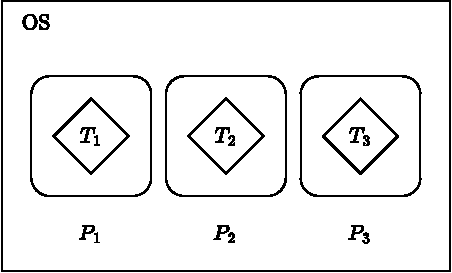
\includegraphics[width=\textwidth]{rozdzialy/rozdzial2/img/processes.pdf}
        \caption{trzy jednowątkowe procesy}
        \label{fig:process-thread-diff:processes}
    \end{subfigure}
    \hfill
    \begin{subfigure}[b]{0.49\textwidth}
        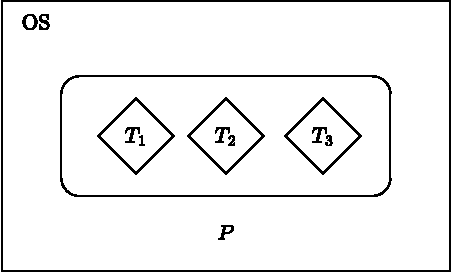
\includegraphics[width=\textwidth]{rozdzialy/rozdzial2/img/threads.pdf}
        \caption{jeden trzywątkowy proces}
        \label{fig:process-thread-diff:threads}
    \end{subfigure}
    \caption{Rozróżnienie procesów i wątków w systemie operacyjnym}
    \source{opracowanie własne na podstawie \cite{tanenbaum2023}}
    \label{fig:process-thread-diff}
\end{figure}

\noindent
Mimo że oba systemy przedstawione powyżej operują na trzech wątkach $T_1$, $T_2$ i~$T_3$, wątki na rysunku \ref{fig:process-thread-diff:processes} operują na odrębnych przestrzeniach adresowych, podczas gdy wątki przedstawione na rysunku \ref{fig:process-thread-diff:threads} działają w obrębie jednej (wspólnej) przestrzeni adresowej, co wynika z faktu operowania wewnątrz jednego (wspólnego) procesu $P$.

% dodac krotki akapit o zasadzie dzialania watkow

\section{Problemy występujące w systemach współbieżnych}
\label{sec:concurrency-problems}
% spisac i opisac najwazniejsze problemy: deadlock, starvation, synchronizacja, sekcja krytyczna, ... (poszukac innych/lepszych)

% race condition, sekcja krytyczna, deadlock, starvation, synchronizacja
% Przeczytac z Goetza poniższe rozdziały: 1.3, cały 2, 5.1, podsumowanie części I (s. 128), 6, 7, 8, 10, 

% mutual exclusion (Ben Ari, 2.2)
% race condition, pamięć współdzielona (rozwiązanie: synchronizacja) (1.3 + 2.2.1)
% problemy żywotności: deadlock (10.1), livelock (10.3.3), starvation (10.3.1) - opisać pojęcie żywotności (1.3.2)
% problemy związane z wydajnością (performance hazards) (1.3.3 + 11)

Mimo wielu zalet wykorzystania wątków do współbieżnego wykonywania zadań, podejście to wiąże się z istnieniem wielu problemów obecnych w systemach współbieżnych. Wiele publikacji wskazuje na cztery główne kategorie problemów: problemy związane z mechanizmem wzajemnego wykluczania i synchronizacją wątków, \emph{race condition} i~pamięć współdzieloną, problemy żywotności, takie jak \emph{deadlock}, \emph{livelock} i \emph{starvation}, a także problemy związane z wydajnością. Poniżej opisano charakterystykę każdego z nich.

\subsection{Wzajemne wykluczanie i synchronizacja}
Ben-Ari \cite{benari1982} definiuje wzajemne wykluczanie (ang. \emph{mutual exclusion}) jako jeden z~najważniejszych problemów programowania współbieżnego z racji bycia abstrakcją dla wielu problemów związanych z synchronizacją wątków.

Herlihy i Shavit \cite{herlihy2012} wskazują, że wątki \emph{wykluczają się wzajemnie}, jeśli co najmniej dwa z nich próbują równocześnie wykonać wspólny blok kodu, nazywany \emph{sekcją krytyczną} (ang. \emph{critical section}), ale w danym momencie tylko jeden z nich ma dostęp do sekcji krytycznej.

% dodać coś jeszcze

\subsection{\emph{Race condition} i pamięć współdzielona}

\subsection{Problemy żywotności: \emph{deadlock}, \emph{livelock}, \emph{starvation}}

Goetz \cite{goetz2006} definiuje \emph{żywotność} (ang. \emph{liveness}) jako właściwość systemu, która zapewnia, że koniec końców pewna własność się wydarzy, czyli że system nie będzie pozostawał w stanie zawieszenia lub bezczynności. Problemy żywotności występują, gdy system nie jest w stanie kontynuować wykonywania zadań z powodu wzajemnych zależności między wątkami lub braku zasobów. Najpopularniejszymi z nich są \emph{deadlock}, \emph{livelock} i \emph{starvation}.

\subsection{Problemy związane z wydajnością}

\section{Modele współbieżności w środowisku JVM}

Środowisko JVM oferuje wiele różnych modeli umożliwiających tworzenie współbieżnych aplikacji. Ta część poświęcona jest omówieniu najpopularniejszych podejść, w tym podstawowego (i chronologicznie pierwszego) modelu, dostępnego w~ramach Thread API, modelu opartego o wykorzystanie wzorca projektowego \emph{Pula} (ang.~\emph{Pool}), dostępnego w ramach interfejsu \texttt{ExecutorService},
% modelu opartego o~framework Fork/Join, realizującego podział zadań i łączenie wyników,
 a~także modelu reaktywnego.

\subsection{Klasyczny model współbieżności (Thread API)}
\label{sec:thread-api}
% okreslenie tego rodzaju watkow jako platform thread, opisac ze watki platformowe w JVM mapuja sie 1:1 na watki OS, opisac wady tego podejscia (tworzenie watku jest kosztowne czasowo i pamieciowo)

\subsection{Model oparty o pule wątków (\texttt{ExecutorService})}
% Goetz 8.2 - rozmiar puli wątków 

% \subsection{Model oparty o podział zadań i łączenie wyników (Fork/Join Framework)}

\subsection{Reaktywny model współbieżności (Reactive Streams, Project Reactor, RxJava)}
\label{sec:reactive}

\cleardoublepage

\chapter{Mechanizmy współbieżności oferowane przez Project Loom}

Trzeci rozdział pracy poświęcony jest omówieniu najważniejszych mechanizmów dostępnych w ramach Project Loom -- inicjatywy usprawniającej tworzenie aplikacji współbieżnych w środowisku JVM. Rozdział zawiera zwięzłą prezentację historii powstawania tego projektu, a także omówienie najważniejszych mechanizmów, które on oferuje, tj. odrębną kategorię wątków, określanych mianem wątków wirtualnych (ang. \emph{virtual threads}), mechanizm współbieżności strukturalnej (ang.~~\emph{structured concurrency}) i~mechanizm przekazywania danych kontekstowych w~ramach zmiennych zakresowych (ang. \emph{scoped values}).
% Rozdział zawiera również omówienie technik integracji mechanizmów oferowanych przez Project Loom z~istniejącymi w~środowisku JVM modelami współbieżności.

\section{Wprowadzenie do Project Loom}

Project Loom jest inicjatywą zapoczątkowaną pod koniec 2017 roku przez OpenJDK. W ramach projektu wyróżnia się trzy główne składowe:
\begin{itemize}
    \item mechanizm \emph{wirtualnych wątków} (ang. \emph{virtual threads}), będący alternatywą dla klasycznego mechanizmu wątków (wątków platformowych) i zdefiniowany w~dokumencie JEP\footnote{JEP (\emph{JDK Enhancement Proposal}) to formalny dokument opisujący proponowane zmiany, nowe funkcjonalności lub usprawnienia platformy JDK.} o numerze 444 \cite{jep444},
    \item mechanizm \emph{współbieżności strukturalnej} (ang. \emph{structured concurrency}), umożliwiający uporządkowanie pracy z wątkami poprzez dodanie tak zwanych \emph{zakresów zadań} (ang. \emph{task scopes}) i strategii zachowań w przypadku wystąpienia błędu lub przerwania działania wątku, opisany w dokumencie JEP~525 \footnote{W chwili publikacji najnowsza wersja mechanizmu współbieżności strukturalnej została udostępniona w wersji \textit{preview}, co oznacza, że jest dostępna w standardowym JDK, lecz jej składnia lub semantyka mogą ulec zmianie przed ostatecznym włączeniem do specyfikacji platformy Java.} \cite{jep525},
    \item mechanizm przekazywania danych kontekstowych między wątkami za pomocą \emph{zmiennych zakresowych} (ang. \emph{scoped values}), będący alternatywą dla klasy \texttt{ThreadLocal} w systemach współbieżnych i opisany w dokumencie JEP~506 \cite{jep506}.
\end{itemize}

Początkowo, ideą projektu było wprowadzenie lekkich wątków użytkownika (ang. \emph{user-mode threads}) oraz uproszczenie programowania współbieżnego, szczególnie w~aplikacjach, których dużą częścią są blokujące zadania, takich jak serwery i~systemy sieciowe \cite{openjdk-loom-proposal}. Wraz z upływem czasu zakres projektu został rozszerzony o mechanizmy zwiększające bezpieczeństwo aplikacji współbieżnych i ustrukturyzowanie pracy z wątkami. Project Loom wciąż ewoluuje, głównie w kontekście zmian w API poszczególnych mechanizmów, lecz większość z nich jest integralną częścią JDK, dodanych w ramach oficjalnych wydań.

\section{Wirtualne wątki (\emph{Virtual Threads})}

Mechanizm wirtualnych wątków, we wczesnych fazach projektu określanych mianem \emph{fibers} \cite{openjdk-loom-proposal}, to chronologicznie pierwsza z trzech głównych składowych projektu Loom, która pod tą nazwą po raz pierwszy pojawiła się w JDK w wersji 19 w~ramach wersji poglądowej (ang. \emph{preview}), a została oficjalnie wydana w ramach JDK 21. Mechanizm ten jest alternatywą dla wątków platformowych, opisanych w~sekcji \hyperref[sec:thread-api]{2.3.1 Klasyczny model współbieżności (Thread API)}.

W celu wyjaśnienia potrzeby wprowadzenia mechanizmu wirtualnych wątków do środowiska JVM, dokument \textit{JEP 444: Virtual Threads} \cite{jep444} powołuje się na prawo Little’a, które wiąże ze sobą latencję, współbieżność i przepustowość w kontekście skalowalności aplikacji współbieżnych:

\begin{displayquote}
    \textit{Dla danego czasu przetwarzania żądania (tj. latencji) liczba żądań obsługiwanych jednocześnie przez aplikację (tj. współbieżność) musi rosnąć proporcjonalnie do tempa napływu żądań (tj. przepustowości).}
\end{displayquote}

\noindent
Jak wspomniano w sekcji \hyperref[sec:thread-api]{2.3.1 Klasyczny model współbieżności (Thread API)}, wątki platformowe w środowisku JVM są zaimplementowane jako obiekty opakowujące (ang. \emph{wrappers}) wątki systemu operacyjnego. Wątki te są zasobożerne, co uniemożliwia ich tworzenie w bardzo dużych ilościach, przez co liczba wątków często staje się czynnikiem ograniczającym skalowalność, na długo przed wyczerpaniem innych zasobów.

Próbą rozwiązania problemu zasobożerności wątków platformowych jest zastosowanie podejścia opartego na współdzieleniu wątków i programowaniu asynchronicznym (patrz sekcja \hyperref[sec:reactive]{2.3.3 Reaktywny model współbieżności (Reactive Streams, Project Reactor, RxJava)}), które umożliwia obsługę dużej liczby współbieżnych operacji przy ograniczonej liczbie wątków systemowych. Rozwiązanie to eliminuje problem kosztowności wątków systemu operacyjnego, jednak odbywa się kosztem znacznego wzrostu złożoności programowania. Asynchroniczny styl wymusza dekompozycję logiki aplikacyjnej na etapy realizowane w postaci wyrażeń lambda, co uniemożliwia wykorzystanie modelu współbieżności obecnego do tej pory w środowisku JVM.

Wirtualne wątki umożliwiają zachowanie paradygmatu \emph{thread-per-request}\footnote{Paradygmat \emph{thread-per-request} zakłada, że każde przychodzące żądanie jest obsługiwane przez dedykowany wątek.} przy jednoczesnym osiągnięciu skalowalności porównywalnej z podejściem asynchronicznym.
% jeszcze parę zdań o tym

\subsubsection{Cykl życia wirtualnych wątków}
% opisac schemat virtual threads <-> carrier threads <-> OS threads
% opisac fakt ze nie warto tworzyć puli VT

Każdorazowo, gdy tworzony jest wirtualny wątek, zostaje on dodany do \emph{kolejki wirtualnych wątków}, będącą kolejką typu FIFO (ang. \emph{First In, First Out}). Wirtualny wątek może wykonać przydzielone mu zadanie, gdy zostanie przypisany do \emph{wątku nośnego} (ang. \emph{carrier thread}). Reprezentuje on wątek platformowy (tj.~wątek systemu operacyjnego) po stronie platformy JVM \cite{veen2024}. Każdy wątek nośny ma przypisany odpowiadający mu wątek platformowy i domyślnie ich liczba jest równa liczbie dostępnych (fizycznych) procesorów logicznych \cite{openjdk-vt-presentation}. W odróżnieniu od~wątków platformowych i nośnych, liczba wirtualnych wątków nie jest zależna od~liczby dostępnych procesorów logicznych, a w większości przypadków ją przekracza. Wynika to ze sposobu zarządzania cyklem ich życia, który został przedstawiony na rysunku \ref{fig:vt-lifecycle}.

\begin{figure}[ht]
    \centering
    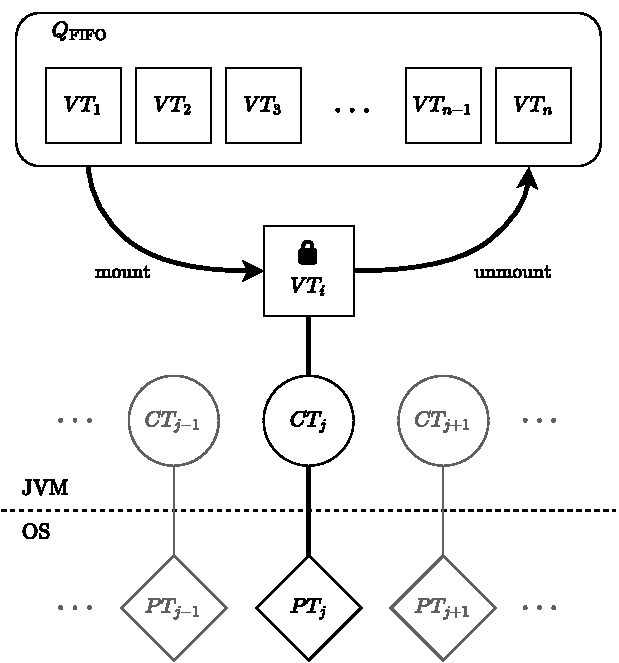
\includegraphics[width=0.75\textwidth]{rozdzialy/rozdzial3/img/VT-lifecycle.pdf}
    \caption{Cykl życia wirtualnych wątków w środowisku JVM}
    \source{opracowanie własne na podstawie \cite{veen2024}}
    \label{fig:vt-lifecycle}
\end{figure}

Korzystając z oznaczeń zawartych na rysunku \ref{fig:vt-lifecycle}, cykl życia wirtualnych wątków w środowisku JVM w kontekście jednego wątku nośnego można opisać następująco:
\begin{enumerate}
    \item Każdy nowy wirtualny wątek $VT$ zostaje dodany na koniec kolejki wirtualnych wątków $Q_{\mathrm{FIFO}}$
    \item Planista (ang. \emph{scheduler}) wątków wirtualnych, obecny w środowisku JVM, bierze pierwszy wolny wątek wirtualny z kolejki przypisuje go (ang. \emph{mount}) do wolnego wątku nośnego ($CT_j$)
    \item Wątek nośny $CT_j$, odpowiadający wątkowi platfomowemu $PT_j$, wykonuje kod przypisany do przydzielonego mu wątku wirtualnego $VT_i$
    \item Gdy wątek wirtualny $VT_i$ wykonuje operację blokującą (stan reprezentowany przez symbol kłódki \faLock), JVM zapisuje jego aktualny stan, dodaje go na koniec kolejki $Q_{\mathrm{FIFO}}$, jednocześnie zwalniając (ang. \emph{unmount}) wątek nośny $CT_j$
    \item JVM przypisuje kolejny wątek wirtualny (tj. pierwszy w kolejce $Q_{\mathrm{FIFO}}$) do wątku nośnego $CT_j$
\end{enumerate}

\section{Współbieżność strukturalna (\emph{Structured Concurrency})}
% doczytać JEP-y
% opisać różnicę: unstructured concurrency vs structured concurrency
% opisać strukturę i działanie StructuredTaskScope

\section{Zmienne zakresowe (\emph{Scoped Values})}
% przeczytać JEP-a

% \section{Integracja mechanizmów Project Loom z~istniejącymi modelami współbieżności}
\cleardoublepage

\chapter{Stan badań i analiza literatury}

\section{Dotychczasowe badania nad Project Loom}

\section{Charakterystyka i wyniki dotychczasowych badań}

\subsection{Obsługa dużej liczby równoczesnych żądań HTTP}

\subsection{Równoległe przetwarzanie złożonych obliczeń}

\section{Zdefiniowanie luki badawczej i kierunku własnych badań}
\cleardoublepage

\chapter{Metodyka badań}

\section{Cel i zakres badań}

\section{Szczegółowy opis scenariuszy testowych}

\subsection{Scenariusz A: Integracja z~bazą danych ze~sterownikiem blokującym (JDBC) i~reaktywnym (R2DBC)}

\subsection{Scenariusz B: Agregacja z użyciem mechanizmu kworum (QS) i propagacją kontekstu}

% \section{Warianty implementacji}

\cleardoublepage

\chapter{Wyniki badań i ich analiza}

% TODO: poprawić po zakończeniu rozdziału
Szósty rozdział pracy przedstawia kryteria oceny wyników badań przeprowadzonych w ramach scenariuszy $\mathcal{A}$ i $\mathcal{B}$, w tym definiuje przyjęte metryki, zawiera szczegółowy opis pomiarów, prezentuje uzyskane wyniki, a także przedstawia ich analizę porównawczą i interpretację.

\section{Kryteria oceny wyników i opis użytych trybów benchmarków}
Badania zdefiniowane w ramach scenariuszy $\mathcal{A}$ i $\mathcal{B}$ przeprowadzono w postaci benchmarków. W tym celu wykorzystano narzędzie Java Microbenchmark Harness (JMH), stanowiące standardowy framework służący do przeprowadzania pomiarów wydajności aplikacji działających w środowisku JVM. Narzędzie to umożliwia wykonywanie powtarzalnych i możliwie precyzyjnych pomiarów czasu wykonania kodu, uwzględniając przy tym specyfikę działania maszyny wirtualnej Java, w~szczególności mechanizmy takie jak kompilacja Just-In-Time (JIT), optymalizacje wykonywanego kodu czy proces rozgrzewania środowiska uruchomieniowego \cite{jmh-source-code}.

\subsection{Tryb pomiaru przepustowości (\texttt{Throughput})}
Tryb \texttt{Throughput} w JMH służy do pomiaru przepustowości badanego fragmentu kodu, określając liczbę operacji wykonanych w jednostce czasu (w przypadku scenariusza $\mathcal{A}$ jednostką czasu jest sekunda). Tryb ten koncentruje się na całkowitej zdolności systemu do przetwarzania zadań przy zadanym obciążeniu, co w badanym scenariuszu pozwoliło na analizę wydajności i skalowalności różnych wariantów systemów współbieżnych. \cite{jmh-documentation}

Z powyższego opisu wynika, że metryką mierzoną przez benchmark uruchomiony w trybie \texttt{Throughput} jest \emph{przepustowość} (ozn. THRPT), czyli liczba operacji wykonanych przez badany fragment kodu w jednostce czasu. Tryb ten został użyty przy pomiarze kodu zaimplementowanego w ramach scenariusza $\mathcal{A}$.

\subsection{Tryb próbkowania czasu (\texttt{SampleTime})}
Tryb \texttt{SampleTime} w JMH służy do pomiaru czasu wykonania pojedynczych wywołań benchmarkowanej metody na podstawie próbek zbieranych w trakcie iteracji pomiarowych.
Wynikiem jest średni czas wykonania operacji wraz z oszacowaniem błędu pomiarowego. Dodatkowo JMH raportuje rozkład zebranych próbek, w tym wartości minimalne i maksymalne oraz percentyle. Wartości te pozwalają ocenić latencję i zachowanie w~ogonie rozkładu \cite{jmh-documentation}. Tryb ten został użyty przy pomiarze kodu zaimplementowanego w ramach obu scenariuszy.

Zgodnie z definicją sformułowaną przez Luszniewicza \cite{luszniewicz1970}, mianem \emph{percentyla rzędu $p$}, gdzie $p \in [0, 100]$, określa się taką wartość $x$, że co najmniej $p\%$ obserwacji ma wartość mniejszą lub równą $x$, a co najwyżej $(100-p)\%$ obserwacji ma wartość większą lub równą $x$.
Na podstawie powyższej definicji, metryką P$n$ określa się percentyl rzędu $n$ czasu wykonania badanego fragmentu kodu. Ponadto, metryką AVG określa się średni czas wykonania badanego fragmentu kodu.

\section{Szczegółowy opis pomiarów}

\subsection{Szczegóły pomiaru dla scenariusza \ensuremath{\mathcal{A}}}
\label{sec:jmh-description-scenario-A}
Każdy z trzech wariantów scenariusza $\mathcal{A}$ (\texttt{JDBC+PT}, \texttt{R2DBC}, \texttt{JDBC+VT}) został uruchomiony dla każdego z trzech zapytań (\texttt{Q1}, \texttt{Q2}, \texttt{Q3}) i na różnych poziomach współbieżności (16, 32, 64, 256, 1024) w następującej konfiguracji narzędzia JMH:
\begin{itemize}
    \itemsep0em
    \item \mintinline{java}|BenchmarkMode| -- tryby benchmarku: \texttt{Throughput} i \texttt{SampleTime},
    \item \mintinline{java}|Warmup| -- liczba iteracji rozgrzewkowych\footnote{Iteracje rozgrzewkowe pozwalają na ustabilizowanie działania środowiska uruchomieniowego JVM, m.in. poprzez aktywację kompilatora JIT i optymalizacji wykonywanego kodu, przed rozpoczęciem właściwych pomiarów. \cite{jmh-documentation}}: 5, każda trwająca 10 sekund,
    \item \mintinline{java}|Measurement| -- liczba iteracji pomiarów właściwych: 10, każda trwająca 10 sekund,
    \item \mintinline{java}|Fork| -- liczba rozgałęzień\footnote{Rozgałęzienia to liczba niezależnych uruchomień środowiska JVM, w których wykonywany jest pomiar. \cite{jmh-documentation}}: 3,
    \item \mintinline{java}|Threads| -- liczba wątków jednocześnie wykonujących kod: 1.
\end{itemize}

\newpage
\noindent
Liczba wątków w powyższej konfiguracji została ustawiona na 1 ze względu na fakt, że zarządzanie liczbą i rodzajem wątków zostało przeniesione bezpośrednio do metod, na których wykonywane są benchmarki. Parametr ten reprezentowany jest przez poziom współbieżności. Implementacja tej logiki różni się w zależności od wariantu modelu współbieżności, co zostało szczegółowo przedstawione w~sekcji \hyperref[sec:results-scenario-A]{5.2.1 Scenariusz \ensuremath{\mathcal{A}}: Integracja z bazą danych ze sterownikiem blokującym (JDBC) i reaktywnym (R2DBC)}.

W celu uniknięcia dokonania niezamierzonych optymalizacji przez środowisko JVM, każdy wariant wykorzystuje wspomniane w rozdziale piątym narzędzie \mintinline{java}|Blackhole| dostępne w ramach JMH, konsumujące wyniki obliczeń w sposób, którego kompilator nie może bezpiecznie zoptymalizować. W ten sposób narzędzie to pozwala zapewnić, że mierzony kod faktycznie zostaje wykonany, a uzyskane wyniki benchmarku odzwierciedlają rzeczywisty koszt obliczeń. \cite{jmh-blackhole}

Metrykami mierzonymi w ramach scenariusza $\mathcal{A}$ są:
\begin{itemize}
    \itemsep0em
    \item dla trybu \texttt{Throughput}: THRPT,
    \item dla trybu \texttt{SampleTime}: AVG, P50, P95 i P99.
\end{itemize}

\subsection{Szczegóły pomiaru dla scenariusza \ensuremath{\mathcal{B}}}
bla bla bla

Metrykami mierzonymi w ramach scenariusza $\mathcal{B}$ są AVG, P50, P95, P99 i P99.9.

\section{Prezentacja wyników pomiarów}

\subsection{Wyniki pomiarów w ramach scenariusza \ensuremath{\mathcal{A}}}
\label{sec:results-scenario-A}

\subsubsection{Tryb pomiaru przepustowości (\texttt{Throughput})}
Tabele \ref{table:benchmark-A-thrpt-Q1}, \ref{table:benchmark-A-thrpt-Q2} i \ref{table:benchmark-A-thrpt-Q3} oraz odpowiadające im wykresy przedstawione na rysunkach \ref{table:benchmark-A-thrpt-Q1}, \ref{table:benchmark-A-thrpt-Q2} i \ref{table:benchmark-A-thrpt-Q3} prezentują wyniki benchmarku przeprowadzonego dla scenariusza $\mathcal{A}$ w~trybie pomiaru przepustowości, tj. w trybie \texttt{Throughput}. Wartości przedstawione w~tabelach i na odpowiadających im wykresach zostały wyznaczone w zależności od wariantu modelu współbieżności, poziomu współbieżności i zapytania.

\noindent
Dodatkowe uwagi do tabel \ref{table:benchmark-A-thrpt-Q1}, \ref{table:benchmark-A-thrpt-Q2} i \ref{table:benchmark-A-thrpt-Q3}:
\begin{enumerate}[label=(\roman*)]
    \itemsep0em
    \item Wyniki we wspomnianych wyżej tabelach podane są jako liczba operacji na sekundę. Wykresy przedstawione na odpowiadających im rysunkach prezentują te dane na osi pionowej w jednostce oznaczonej jako [ops/s].
    \item Wyniki we wspomnianych wyżej tabelach przedstawione są w formacie $S \pm E$, gdzie $S$~oznacza uzyskany wynik, a~$E$ oznacza błąd pomiaru.
    \item Wyniki i wartości błędów pomiaru we wspomnianych wyżej tabelach zapisane zostały z kropką jako separatorem dziesiętnym i zmierzone z dokładnością do części tysięcznych, tj. $0.001$.
\end{enumerate}

\vspace{3cm}
\textit{Wyniki znajdują się na następnej stronie.}

\begin{figure}[p]
    \centering
    \setlength{\tabcolsep}{0.5em}
    \renewcommand{\arraystretch}{1.2}
    \begin{tabularx}{\linewidth}{|c|>{\centering\arraybackslash}X|>{\centering\arraybackslash}X|>{\centering\arraybackslash}X|}
        \hline
        \textbf{Poz. współb.} & \textbf{JDBC+PT} & \textbf{R2DBC} & \textbf{JDBC+VT} \\
        \hline
        16 & $415.881 \pm 8.497$ & $729.356 \pm 5.935$ & $733.642 \pm 13.414$ \\
        \hline
        32 & $230.098 \pm 7.511$ & $451.219 \pm 2.474$ & $489.411 \pm 2.623$ \\
        \hline
        64 & $116.672 \pm 4.463$ & $240.370 \pm 4.193$ & $250.862 \pm 0.876$ \\
        \hline
        256 & $28.871 \pm 1.067$ & $67.178 \pm 0.352$ & $66.336 \pm 0.378$ \\
        \hline
        1024 & $6.694 \pm 0.306$ & $17.139 \pm 0.105$ & $16.782 \pm 0.111$ \\
        \hline
    \end{tabularx}
    \captionof{table}{Wartości przepustowości dla zapytania \texttt{Q1} w~ramach scenariusza $\mathcal{A}$ w~zależności od poziomu współbieżności i wariantu modelu współbieżności}
    \source{opracowanie własne}
    \label{table:benchmark-A-thrpt-Q1}
    \vspace{0.5cm} % Odstęp między tabelą a wykresami

    % --- WYKRESY ---
    \begin{subfigure}[b]{0.49\textwidth}
        \centering
        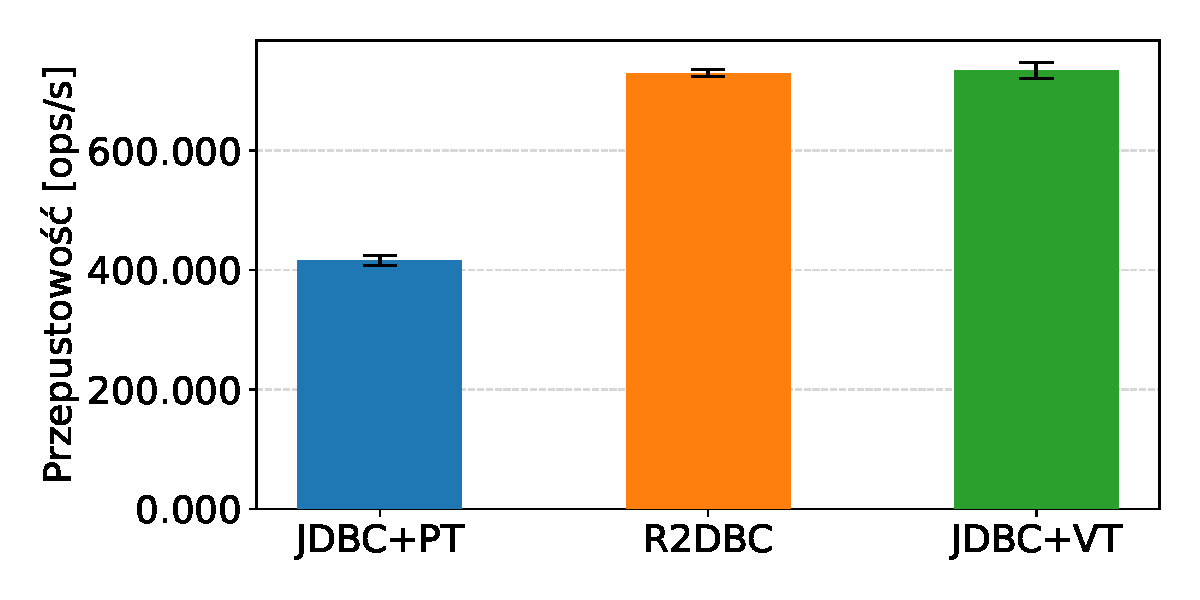
\includegraphics[width=\textwidth]{rozdzialy/rozdzial6/wykresy/A_plot_thrpt_Q1_16.pdf}
        \caption{poziom współbieżności: 16}
    \end{subfigure}
    \hfill
    \begin{subfigure}[b]{0.49\textwidth}
        \centering
        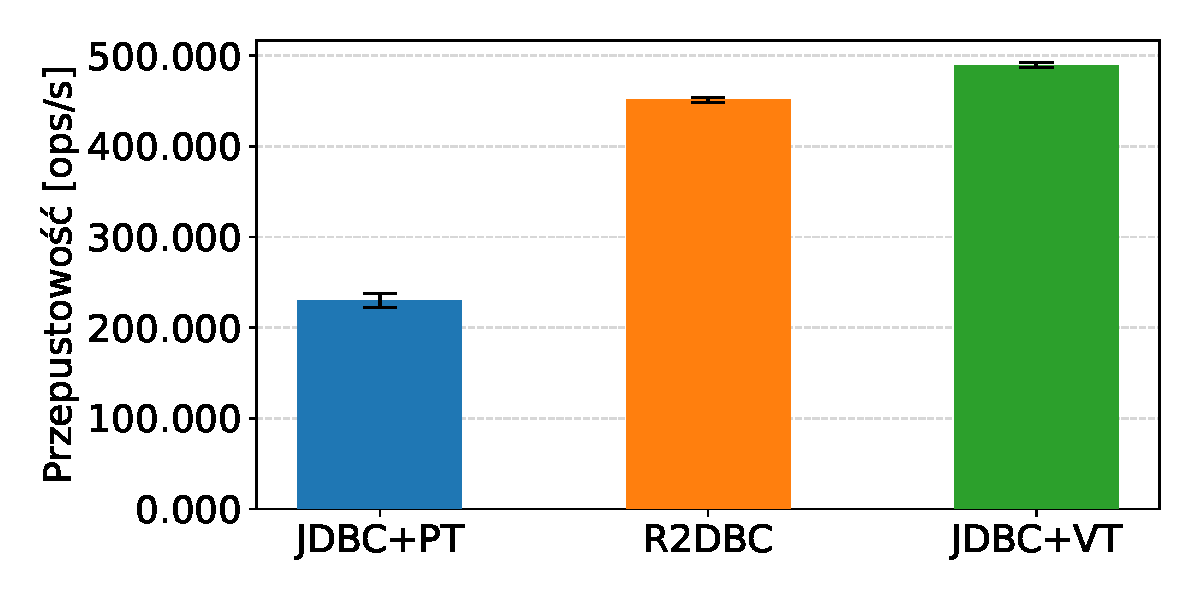
\includegraphics[width=\textwidth]{rozdzialy/rozdzial6/wykresy/A_plot_thrpt_Q1_32.pdf}
        \caption{poziom współbieżności: 32}
    \end{subfigure}

    \vspace{0.2cm}

    \begin{subfigure}[b]{0.49\textwidth}
        \centering
        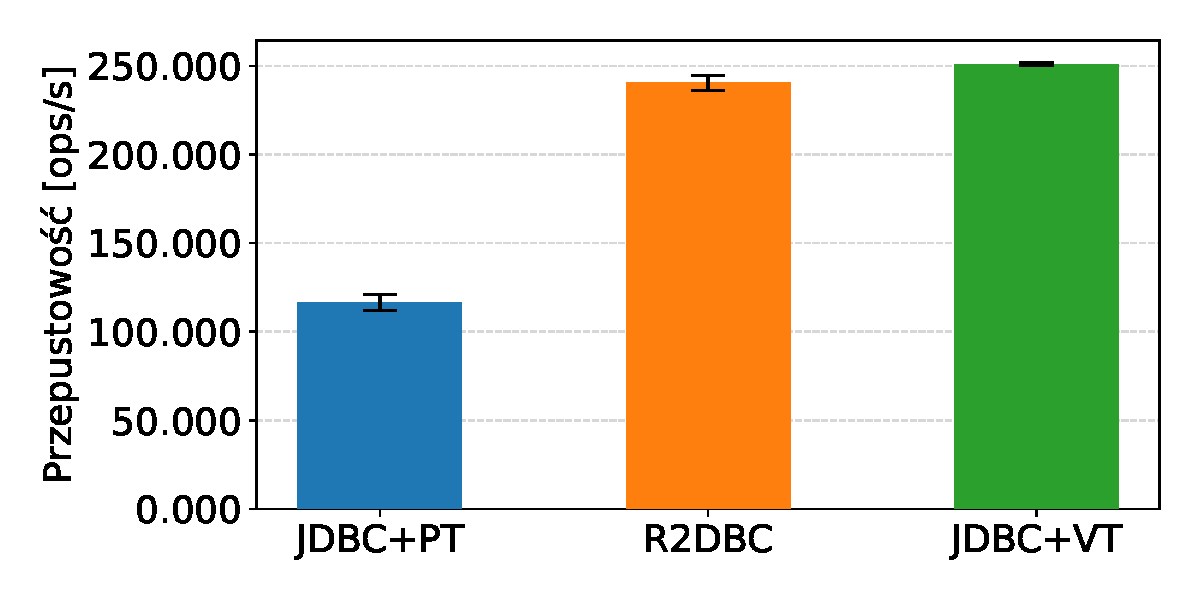
\includegraphics[width=\textwidth]{rozdzialy/rozdzial6/wykresy/A_plot_thrpt_Q1_64.pdf}
        \caption{poziom współbieżności: 64}
    \end{subfigure}
    \hfill
    \begin{subfigure}[b]{0.49\textwidth}
        \centering
        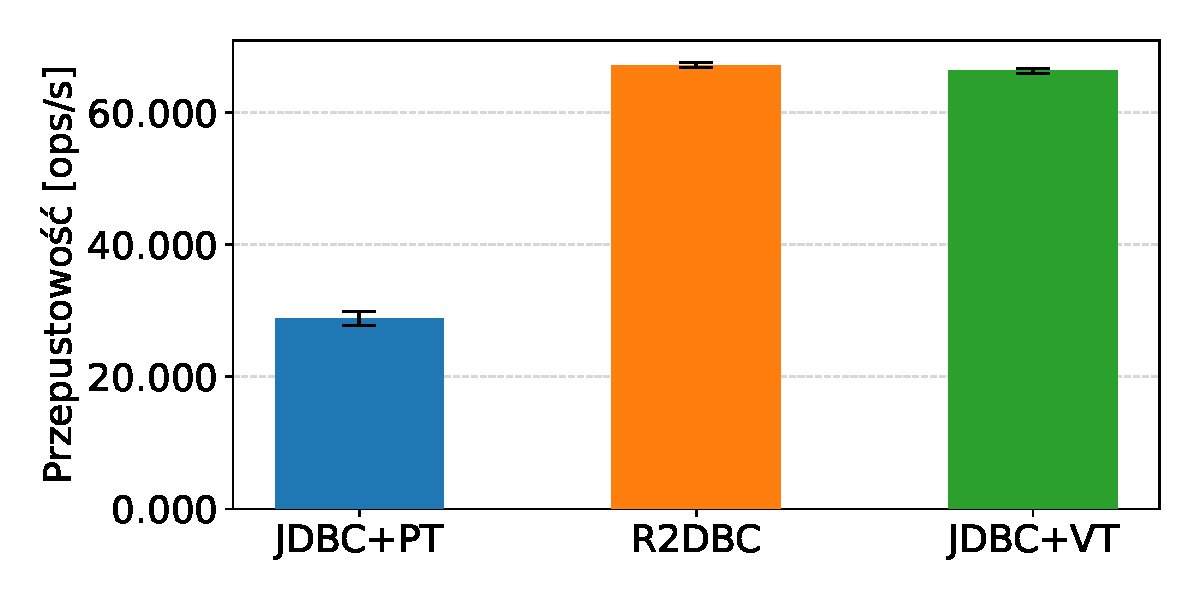
\includegraphics[width=\textwidth]{rozdzialy/rozdzial6/wykresy/A_plot_thrpt_Q1_256.pdf}
        \caption{poziom współbieżności: 256}
    \end{subfigure}

    \vspace{0.2cm}

    \begin{subfigure}[b]{0.49\textwidth}
        \centering
        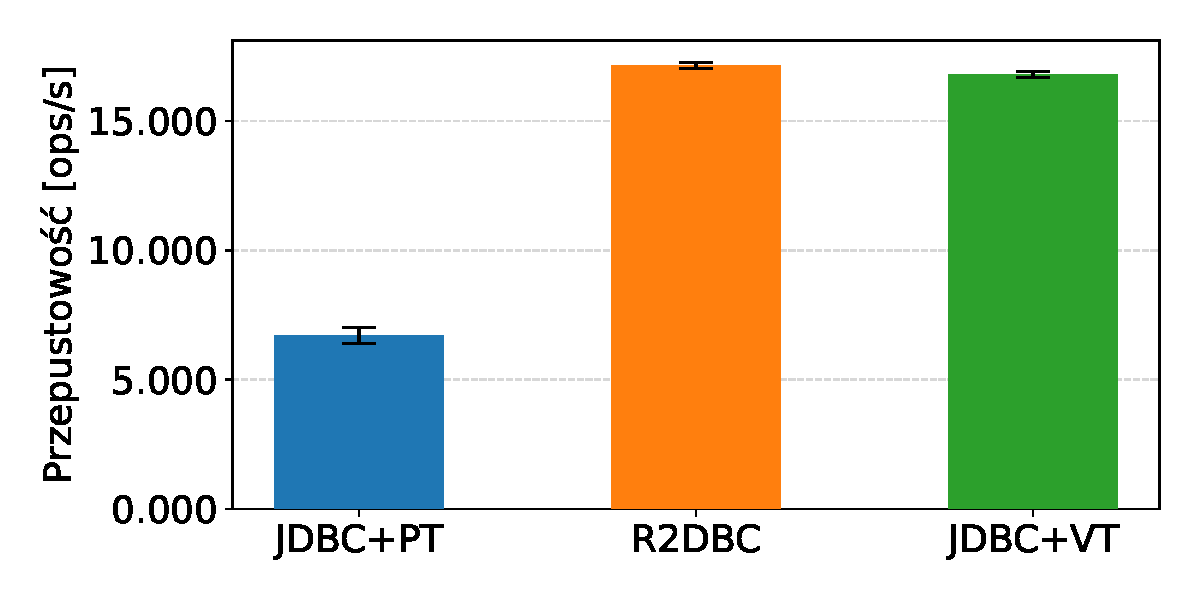
\includegraphics[width=\textwidth]{rozdzialy/rozdzial6/wykresy/A_plot_thrpt_Q1_1024.pdf}
        \caption{poziom współbieżności: 1024}
    \end{subfigure}

    \captionof{figure}{Wykresy kolumnowe przepustowości dla zapytania \texttt{Q1} w ramach scenariusza $\mathcal{A}$ w zależności od poziomu współbieżności i wariantu modelu współbieżności}
    \source{opracowanie własne}
    \label{fig:benchmark-A-thrpt-Q1}
\end{figure}

\begin{figure}[p]
    \centering
    \setlength{\tabcolsep}{0.5em}
    \renewcommand{\arraystretch}{1.2}
    \begin{tabularx}{\linewidth}{|c|>{\centering\arraybackslash}X|>{\centering\arraybackslash}X|>{\centering\arraybackslash}X|}
        \hline
        \textbf{Poz. współb.} & \textbf{JDBC+PT} & \textbf{R2DBC} & \textbf{JDBC+VT} \\
        \hline
        16 & $142.817 \pm 24.898$ & $174.474 \pm 36.850$ & $159.069 \pm 33.964$ \\
        \hline
        32 & $107.766 \pm 14.097$ & $122.683 \pm 0.635$ & $157.456 \pm 29.941$ \\
        \hline
        64 & $55.572 \pm 5.507$ & $74.120 \pm 10.150$ & $70.235 \pm 4.447$ \\
        \hline
        256 & $14.765 \pm 1.268$ & $19.392 \pm 2.232$ & $19.884 \pm 1.825$ \\
        \hline
        1024 & $3.736 \pm 0.365$ & $4.600 \pm 0.031$ & $5.042 \pm 0.379$ \\
        \hline
    \end{tabularx}
    \captionof{table}{Wartości przepustowości dla zapytania \texttt{Q2} w ramach scenariusza $\mathcal{A}$ w~zależności od poziomu współbieżności i wariantu modelu współbieżności}
    \source{opracowanie własne}
    \label{table:benchmark-A-thrpt-Q2}
    \vspace{0.5cm} % Odstęp między tabelą a wykresami

    % --- WYKRESY ---
    \begin{subfigure}[b]{0.49\textwidth}
        \centering
        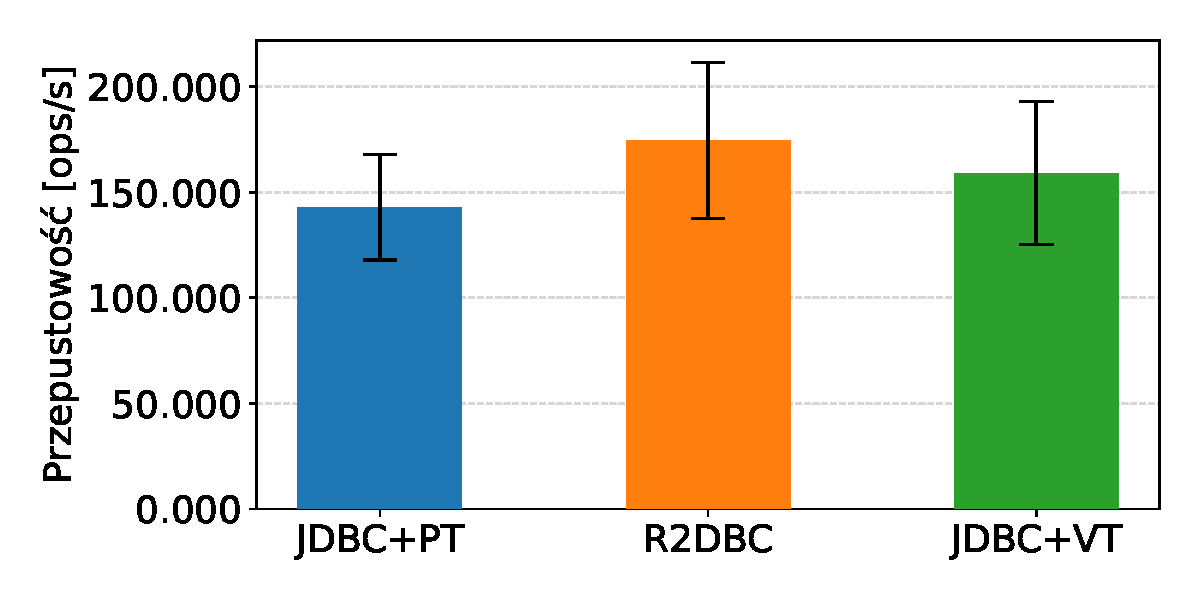
\includegraphics[width=\textwidth]{rozdzialy/rozdzial6/wykresy/A_plot_thrpt_Q2_16.pdf}
        \caption{poziom współbieżności: 16}
    \end{subfigure}
    \hfill
    \begin{subfigure}[b]{0.49\textwidth}
        \centering
        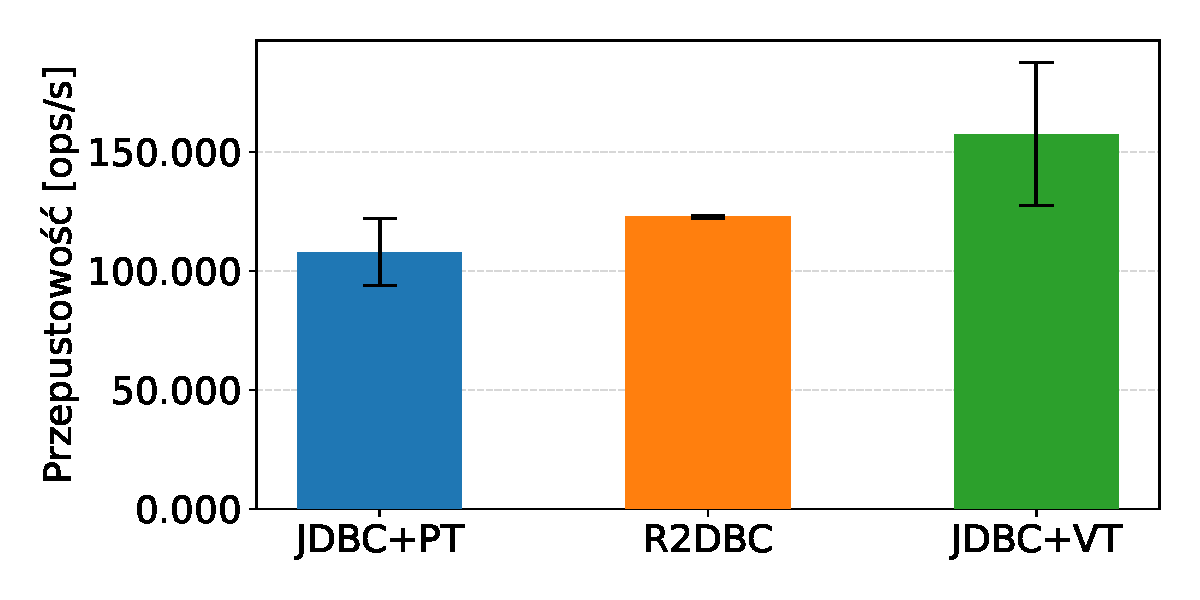
\includegraphics[width=\textwidth]{rozdzialy/rozdzial6/wykresy/A_plot_thrpt_Q2_32.pdf}
        \caption{poziom współbieżności: 32}
    \end{subfigure}

    \vspace{0.2cm}

    \begin{subfigure}[b]{0.49\textwidth}
        \centering
        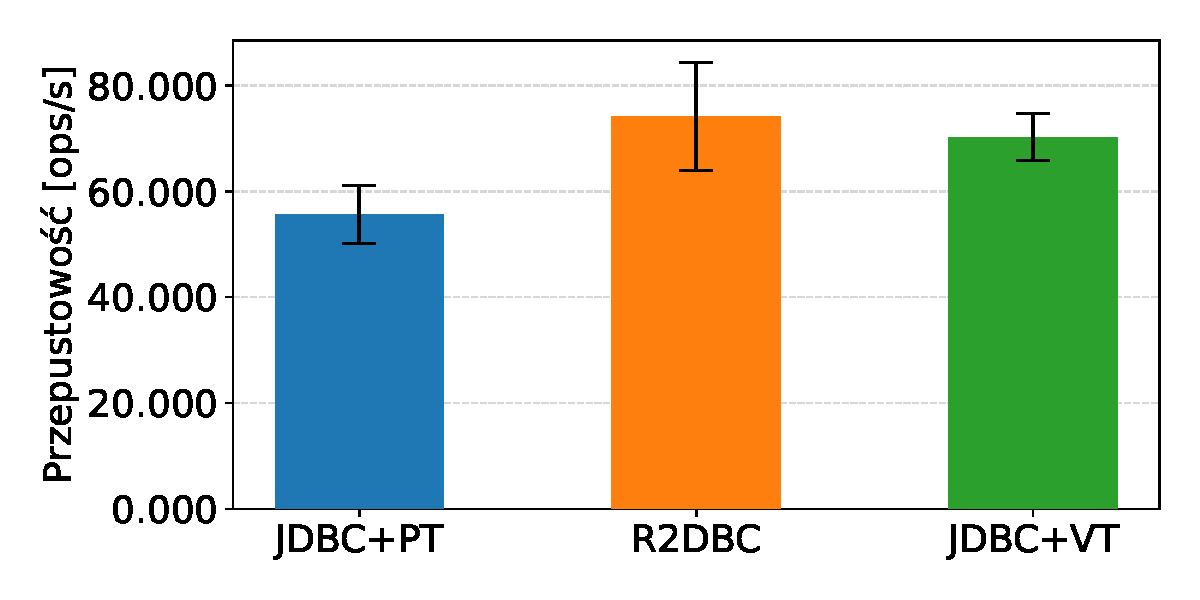
\includegraphics[width=\textwidth]{rozdzialy/rozdzial6/wykresy/A_plot_thrpt_Q2_64.pdf}
        \caption{poziom współbieżności: 64}
    \end{subfigure}
    \hfill
    \begin{subfigure}[b]{0.49\textwidth}
        \centering
        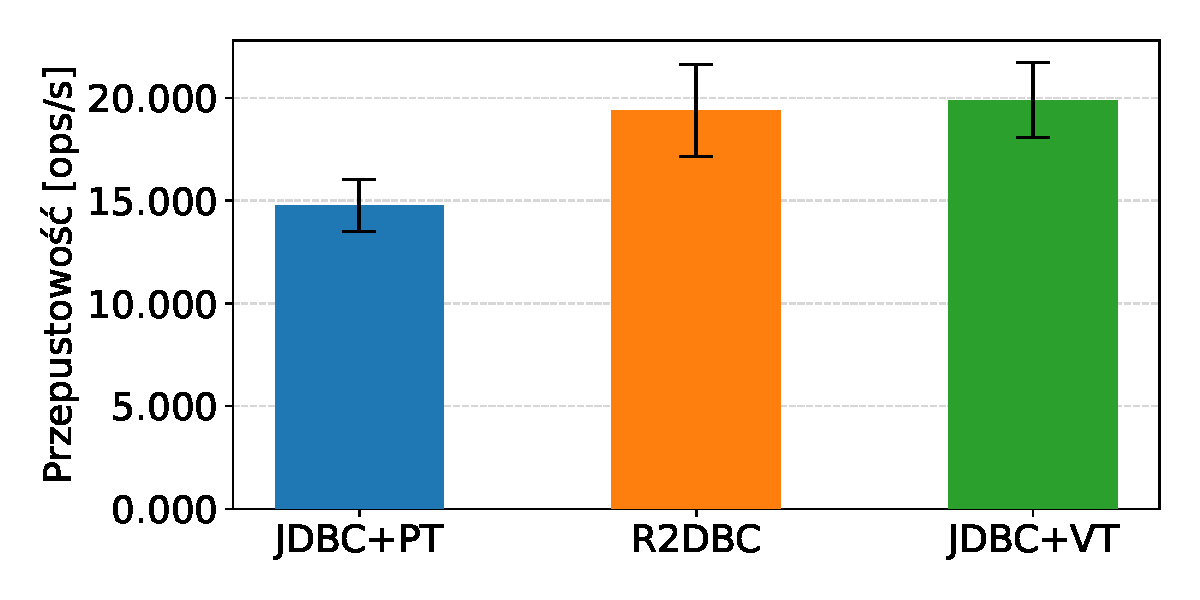
\includegraphics[width=\textwidth]{rozdzialy/rozdzial6/wykresy/A_plot_thrpt_Q2_256.pdf}
        \caption{poziom współbieżności: 256}
    \end{subfigure}

    \vspace{0.2cm}

    \begin{subfigure}[b]{0.49\textwidth}
        \centering
        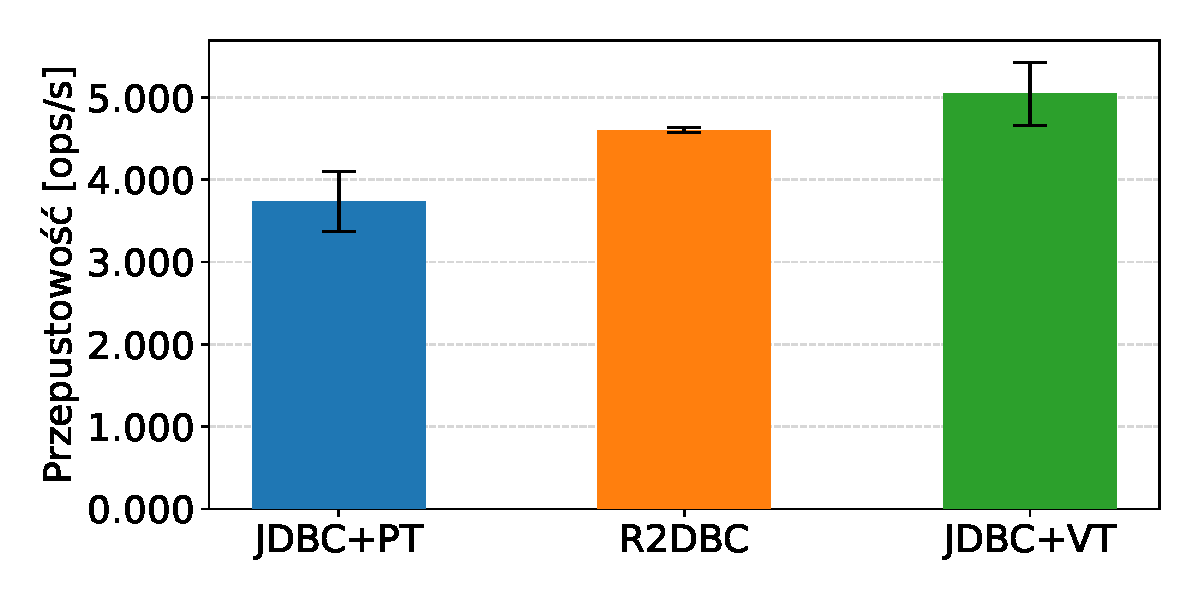
\includegraphics[width=\textwidth]{rozdzialy/rozdzial6/wykresy/A_plot_thrpt_Q2_1024.pdf}
        \caption{poziom współbieżności: 1024}
    \end{subfigure}

    \captionof{figure}{Wykresy kolumnowe przepustowości dla zapytania \texttt{Q2} w ramach scenariusza $\mathcal{A}$ w zależności od poziomu współbieżności i wariantu modelu współbieżności}
    \source{opracowanie własne}
    \label{fig:benchmark-A-thrpt-Q2}
\end{figure}

\begin{figure}[p]
    \centering
    \setlength{\tabcolsep}{0.5em}
    \renewcommand{\arraystretch}{1.2}
    \begin{tabularx}{\linewidth}{|c|>{\centering\arraybackslash}X|>{\centering\arraybackslash}X|>{\centering\arraybackslash}X|}
        \hline
        \textbf{Poz. współb.} & \textbf{JDBC+PT} & \textbf{R2DBC} & \textbf{JDBC+VT} \\
        \hline
        16 & $4.943 \pm 0.020$ & $5.003 \pm 0.027$ & $4.940 \pm 0.027$ \\
        \hline
        32 & $2.667 \pm 0.009$ & $2.705 \pm 0.011$ & $2.673 \pm 0.010$ \\
        \hline
        64 & $1.319 \pm 0.004$ & $1.332 \pm 0.006$ & $1.314 \pm 0.008$ \\
        \hline
        256 & $0.330 \pm 0.002$ & $0.335 \pm 0.001$ & $0.330 \pm 0.002$ \\
        \hline
        1024 & $0.187 \pm 0.001$ & $0.084 \pm 0.001$ & $0.192 \pm 0.001$ \\
        \hline
    \end{tabularx}
    \captionof{table}{Wartości przepustowości dla zapytania \texttt{Q3} w ramach scenariusza $\mathcal{A}$ w~zależności od poziomu współbieżności i wariantu modelu współbieżności}
    \source{opracowanie własne}
    \label{table:benchmark-A-thrpt-Q3}

    \vspace{0.5cm} % Odstęp między tabelą a wykresami

    % --- WYKRESY ---
    \begin{subfigure}[b]{0.49\textwidth}
        \centering
        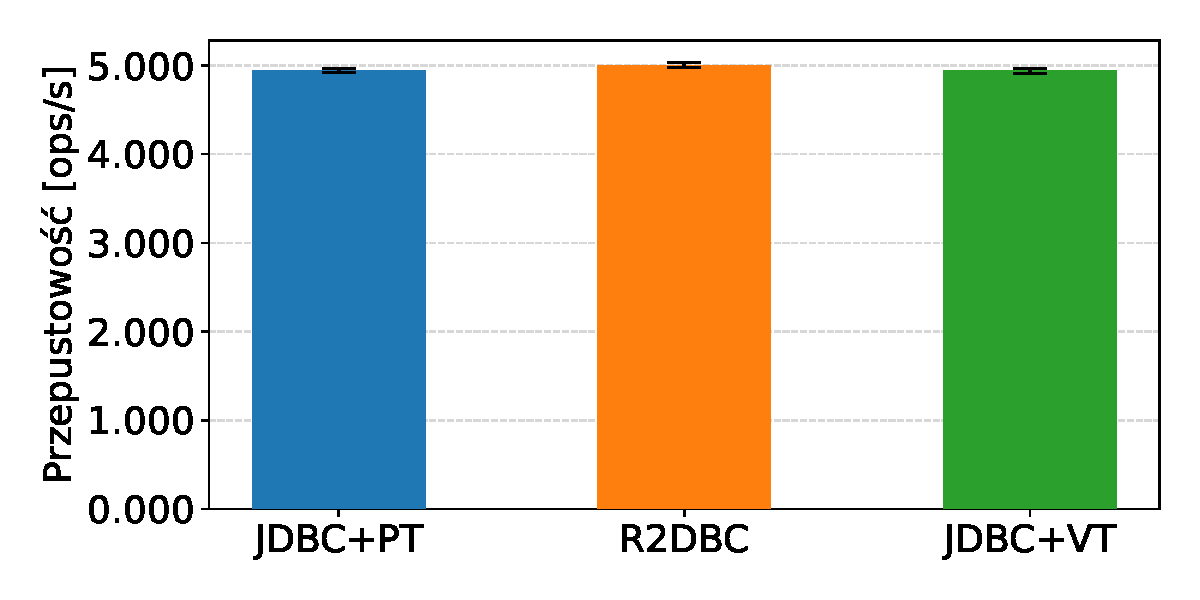
\includegraphics[width=\textwidth]{rozdzialy/rozdzial6/wykresy/A_plot_thrpt_Q3_16.pdf}
        \caption{poziom współbieżności: 16}
    \end{subfigure}
    \hfill
    \begin{subfigure}[b]{0.49\textwidth}
        \centering
        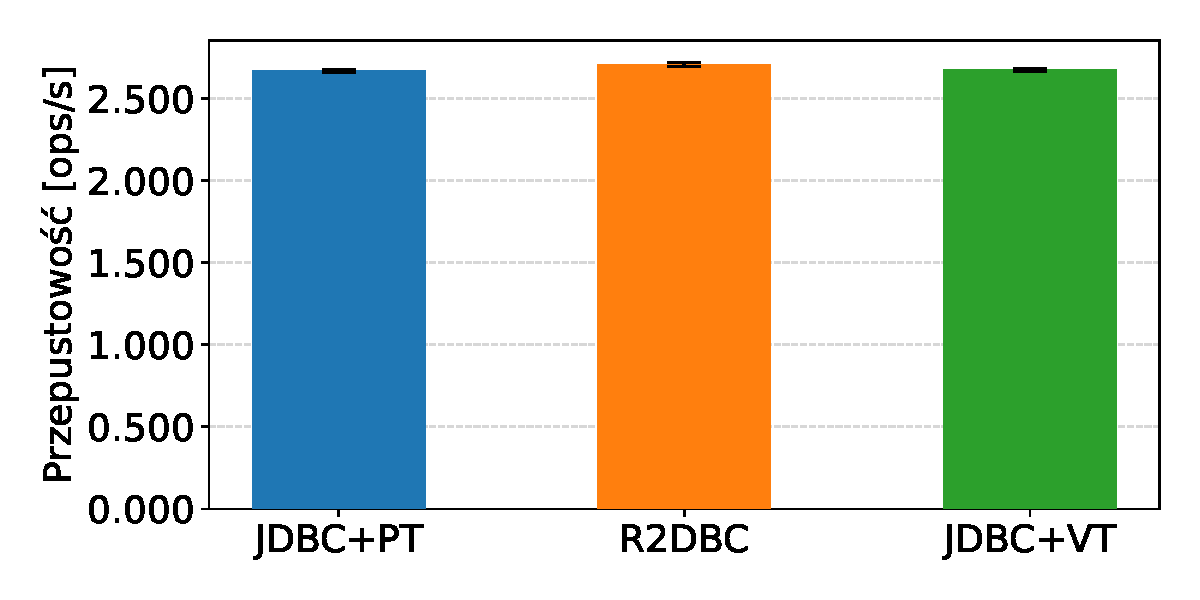
\includegraphics[width=\textwidth]{rozdzialy/rozdzial6/wykresy/A_plot_thrpt_Q3_32.pdf}
        \caption{poziom współbieżności: 32}
    \end{subfigure}

    \vspace{0.2cm}

    \begin{subfigure}[b]{0.49\textwidth}
        \centering
        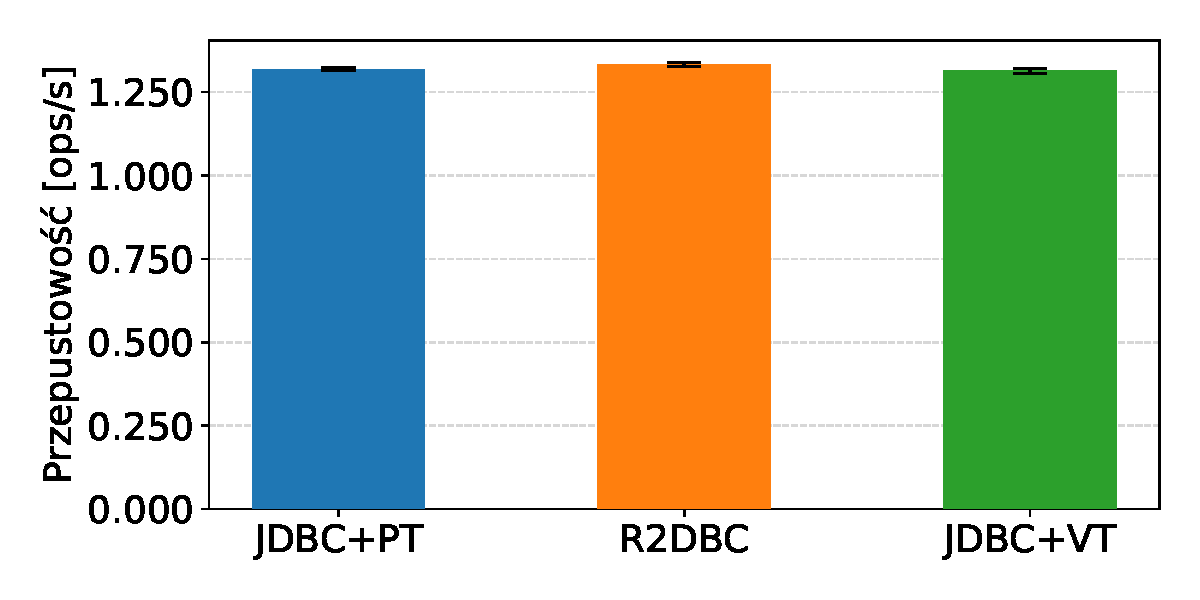
\includegraphics[width=\textwidth]{rozdzialy/rozdzial6/wykresy/A_plot_thrpt_Q3_64.pdf}
        \caption{poziom współbieżności: 64}
    \end{subfigure}
    \hfill
    \begin{subfigure}[b]{0.49\textwidth}
        \centering
        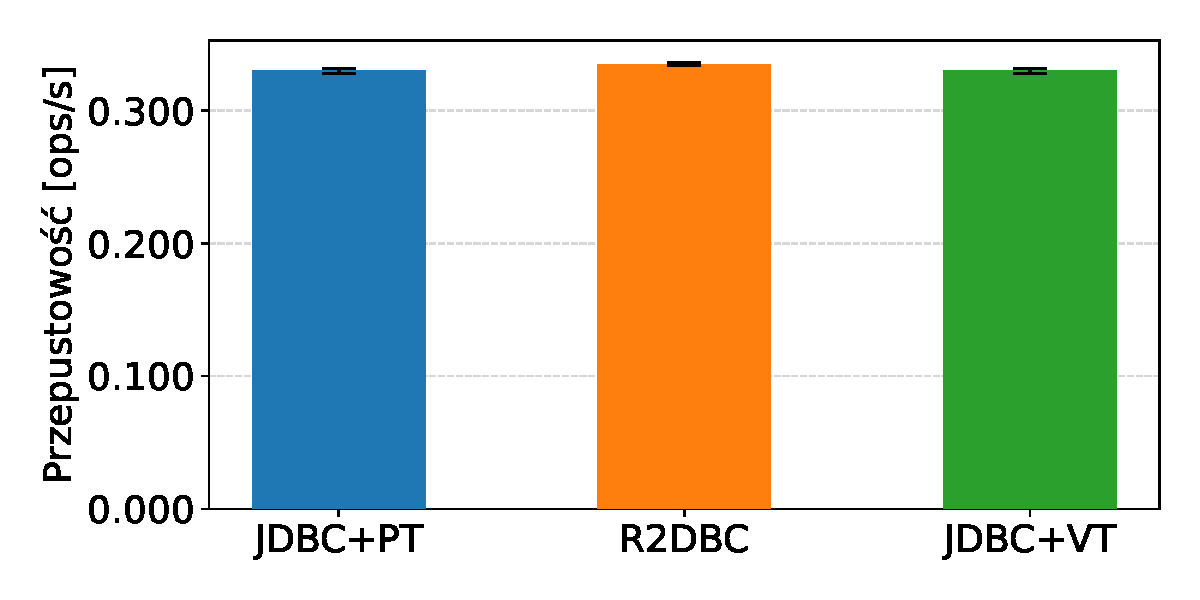
\includegraphics[width=\textwidth]{rozdzialy/rozdzial6/wykresy/A_plot_thrpt_Q3_256.pdf}
        \caption{poziom współbieżności: 256}
    \end{subfigure}

    \vspace{0.2cm}

    \begin{subfigure}[b]{0.49\textwidth}
        \centering
        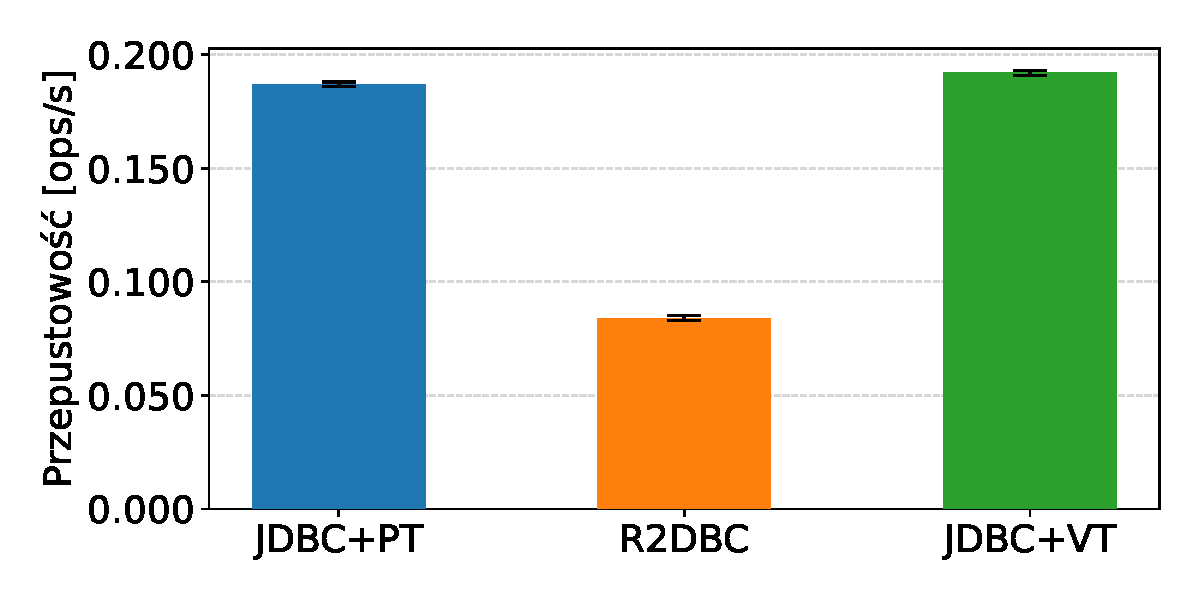
\includegraphics[width=\textwidth]{rozdzialy/rozdzial6/wykresy/A_plot_thrpt_Q3_1024.pdf}
        \caption{poziom współbieżności: 1024}
    \end{subfigure}

    \captionof{figure}{Wykresy kolumnowe przepustowości dla zapytania \texttt{Q3} w ramach scenariusza $\mathcal{A}$ w zależności od poziomu współbieżności i wariantu modelu współbieżności}
    \source{opracowanie własne}
    \label{fig:benchmark-A-thrpt-Q3}
\end{figure}

\newpage
\subsubsection{Tryb próbkowania czasu (\texttt{SampleTime})}

Dodatkowe uwagi do tabel \ref{table:benchmark-A-sample-Q1}, \ref{table:benchmark-A-sample-Q2} i \ref{table:benchmark-A-sample-Q3}:
\begin{enumerate}[label=(\roman*)]
    \item Wyniki we wspomnianych wyżej tabelach uwzględniają średni czas (AVG) i wartości percentyli P50, P95, P99 czasu wykonania badanych wariantów scenariusza i podane są w sekundach. Wykresy przedstawione na na odpowiadających im rysunkach prezentują te dane na osi pionowej w jednostce oznaczonej jako [s].
    \item Wyniki we wierszach oznaczonych przez AVG we wspomnianych wyżej tabelach są przedstawione w formacie $S \pm E$, gdzie $S$ oznacza uzyskany wynik, a~$E$ oznacza błąd pomiaru.
    \item Wyniki i wartości błędów we wspomnianych wyżej tabelach zapisane zostały z kropką jako separatorem dziesiętnym, z dokładnością do części tysięcznych, tj. $0.001$.
\end{enumerate}

\vspace{3cm}
\textit{Wyniki znajdują się na następnej stronie.}

\setlength{\tabcolsep}{0.5em} % for the horizontal padding
\renewcommand{\arraystretch}{1.2} % for the vertical padding
\begin{table}[p]
    \centering
    \setlength{\tabcolsep}{0.5em}
    \renewcommand{\arraystretch}{1.2}
    \begin{tabularx}{\linewidth}{|c|c|>{\centering\arraybackslash}X|>{\centering\arraybackslash}X|>{\centering\arraybackslash}X|}
        \hline
        \textbf{Poz. współb.} & \textbf{Metryka} & \textbf{JDBC + PT} & \textbf{R2DBC} & \textbf{JDBC + VT} \\
        \hline
        \multirow{4}{*}{16} & AVG & $0.003 \pm 0.001$ & $0.001 \pm 0.001$ & $0.001 \pm 0.001$ \\ \cline{2-5}
                            & P50 & 0.003 & 0.001 & 0.001 \\ \cline{2-5}
                            & P95 & 0.003 & 0.002 & 0.002 \\ \cline{2-5}
                            & P99 & 0.004 & 0.002 & 0.002 \\
        \hline
        \multirow{4}{*}{32} & AVG & $0.004 \pm 0.001$ & $0.002 \pm 0.001$ & $0.002 \pm 0.001$ \\ \cline{2-5}
                            & P50 & 0.004 & 0.002 & 0.002 \\ \cline{2-5}
                            & P95 & 0.005 & 0.003 & 0.002 \\ \cline{2-5}
                            & P99 & 0.006 & 0.004 & 0.003 \\
        \hline
        \multirow{4}{*}{64} & AVG & $0.009 \pm 0.001$ & $0.004 \pm 0.001$ & $0.004 \pm 0.001$ \\ \cline{2-5}
                            & P50 & 0.009 & 0.004 & 0.004 \\ \cline{2-5}
                            & P95 & 0.010 & 0.005 & 0.005 \\ \cline{2-5}
                            & P99 & 0.011 & 0.006 & 0.006 \\
        \hline
        \multirow{4}{*}{256} & AVG & $0.036 \pm 0.001$ & $0.015 \pm 0.001$ & $0.015 \pm 0.001$ \\ \cline{2-5}
                             & P50 & 0.035 & 0.015 & 0.015 \\ \cline{2-5}
                             & P95 & 0.039 & 0.017 & 0.018 \\ \cline{2-5}
                             & P99 & 0.043 & 0.020 & 0.020 \\
        \hline
        \multirow{4}{*}{1024} & AVG & $0.159 \pm 0.001$ & $0.058 \pm 0.001$ & $0.060 \pm 0.001$ \\ \cline{2-5}
                              & P50 & 0.158 & 0.057 & 0.058 \\ \cline{2-5}
                              & P95 & 0.177 & 0.065 & 0.066 \\ \cline{2-5}
                              & P99 & 0.187 & 0.070 & 0.071 \\
        \hline
    \end{tabularx}
    \caption{Wartości średniego czasu i percentyli P50, P95, P99 dla zapytania \texttt{Q1} w~ramach scenariusza $\mathcal{A}$ w~zależności od poziomu współbieżności i~wariantu modelu współbieżności}
    \source{opracowanie własne}
    \label{table:benchmark-A-sample-Q1}
\end{table}

    % \begin{subfigure}[b]{0.49\textwidth}
    %     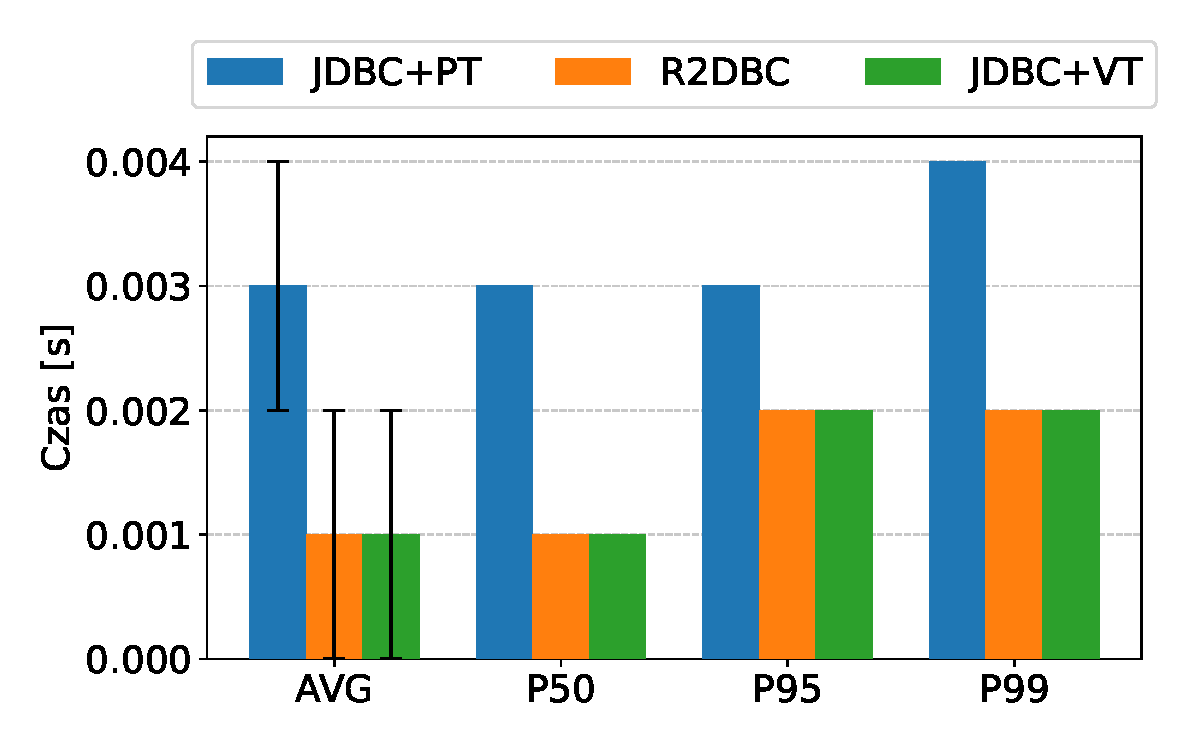
\includegraphics[width=\textwidth]{rozdzialy/rozdzial6/wykresy/A_plot_avg_Q1_16.pdf}
    %     \caption{poziom współbieżności: 16}
    %     \label{fig:benchmark-A-sample-Q1-16}
    % \end{subfigure}
    % \hfill
    % \begin{subfigure}[b]{0.49\textwidth}
    %     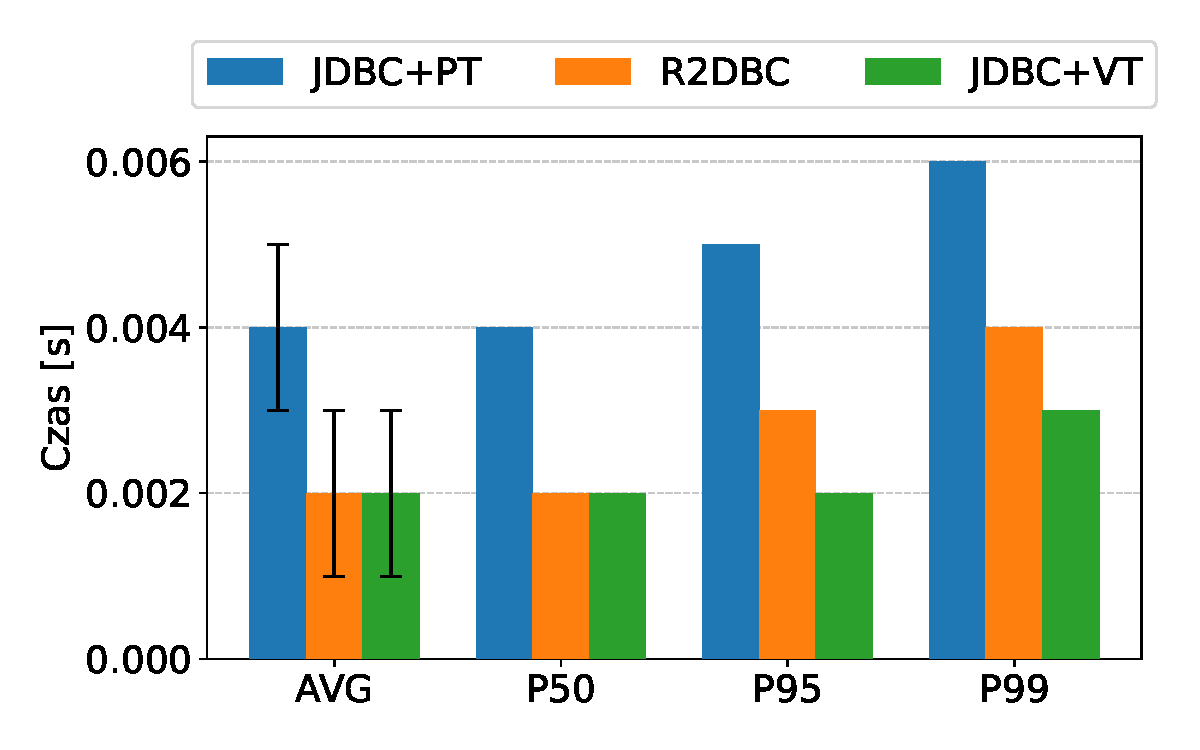
\includegraphics[width=\textwidth]{rozdzialy/rozdzial6/wykresy/A_plot_avg_Q1_32.pdf}
    %     \caption{poziom współbieżności: 32}
    %     \label{fig:benchmark-A-sample-Q1-32}
    % \end{subfigure}

    % \vspace{0.5cm}

    % \begin{subfigure}[b]{0.49\textwidth}
    %     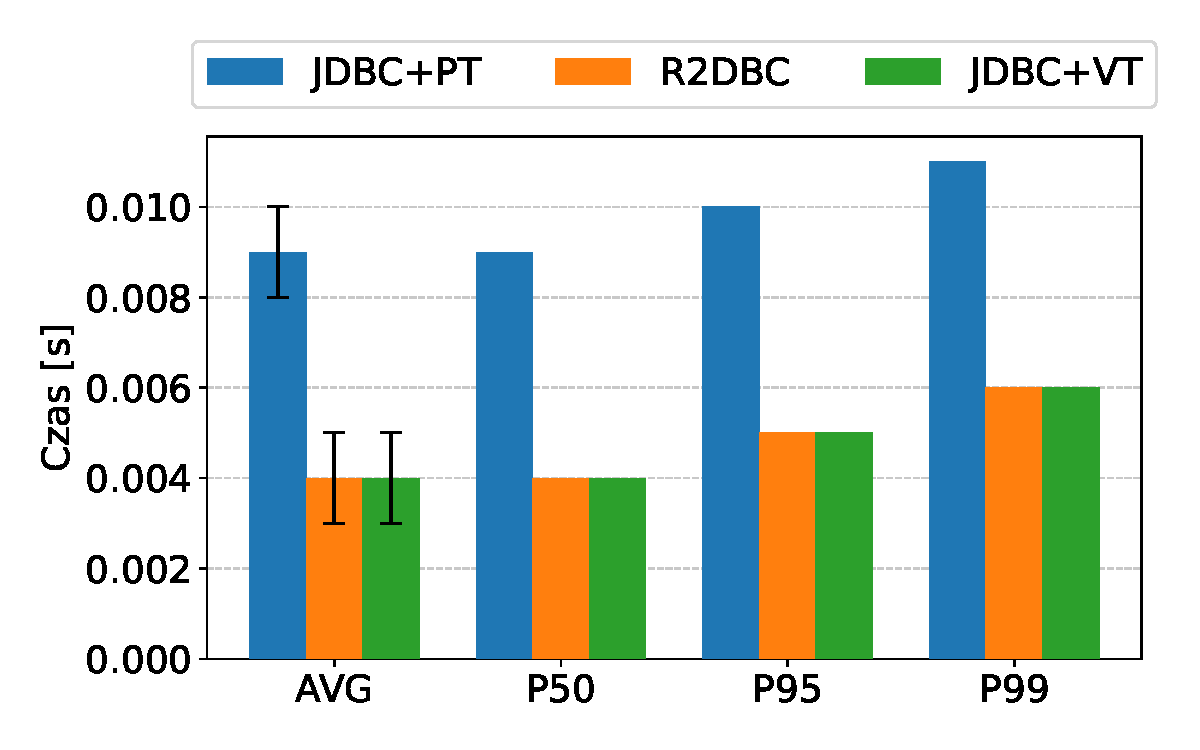
\includegraphics[width=\textwidth]{rozdzialy/rozdzial6/wykresy/A_plot_avg_Q1_64.pdf}
    %     \caption{poziom współbieżności: 64}
    %     \label{fig:benchmark-A-sample-Q1-64}
    % \end{subfigure}
    % \hfill
    % \begin{subfigure}[b]{0.49\textwidth}
    %     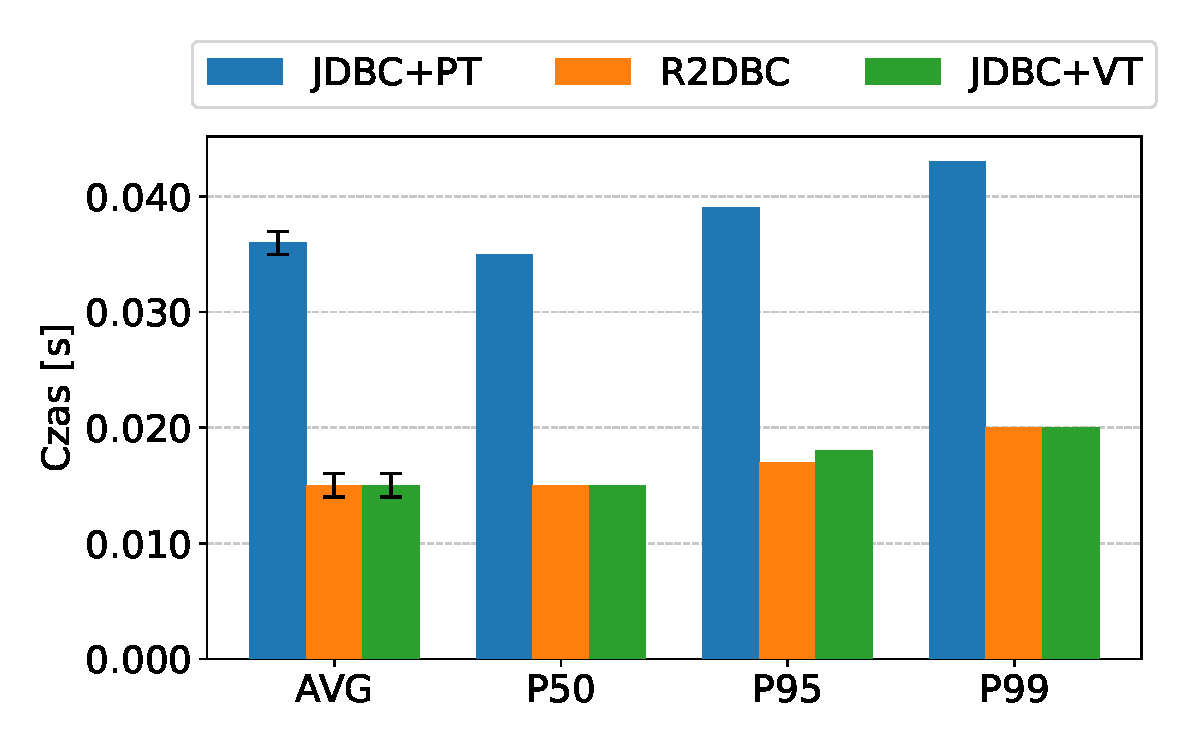
\includegraphics[width=\textwidth]{rozdzialy/rozdzial6/wykresy/A_plot_avg_Q1_256.pdf}
    %     \caption{poziom współbieżności: 256}
    %     \label{fig:benchmark-A-sample-Q1-256}
    % \end{subfigure}

    % \vspace{0.5cm}

    % \begin{subfigure}[b]{0.49\textwidth}
    %     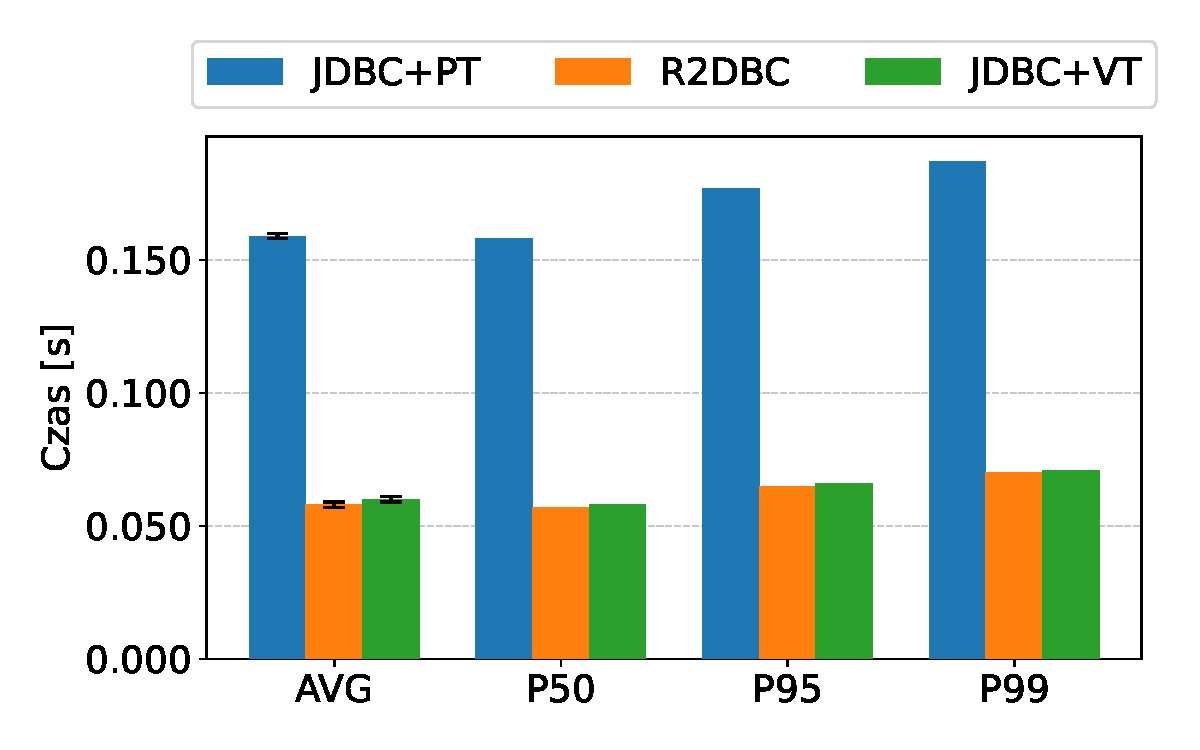
\includegraphics[width=\textwidth]{rozdzialy/rozdzial6/wykresy/A_plot_avg_Q1_1024.pdf}
    %     \caption{poziom współbieżności: 1024}
    %     \label{fig:benchmark-A-sample-Q1-1024}
    % \end{subfigure}
    % \captionof{figure}{Wykresy kolumnowe średniego czasu i latencji P50, P95, P99 dla różnych modeli współbieżności w scenariuszu A dla zapytania \texttt{Q1}}
    % \source{opracowanie własne}
    % \label{fig:benchmark-A-sample-Q1}

\begin{figure}[p]
    \centering
    \begin{subfigure}[b]{0.49\textwidth}
        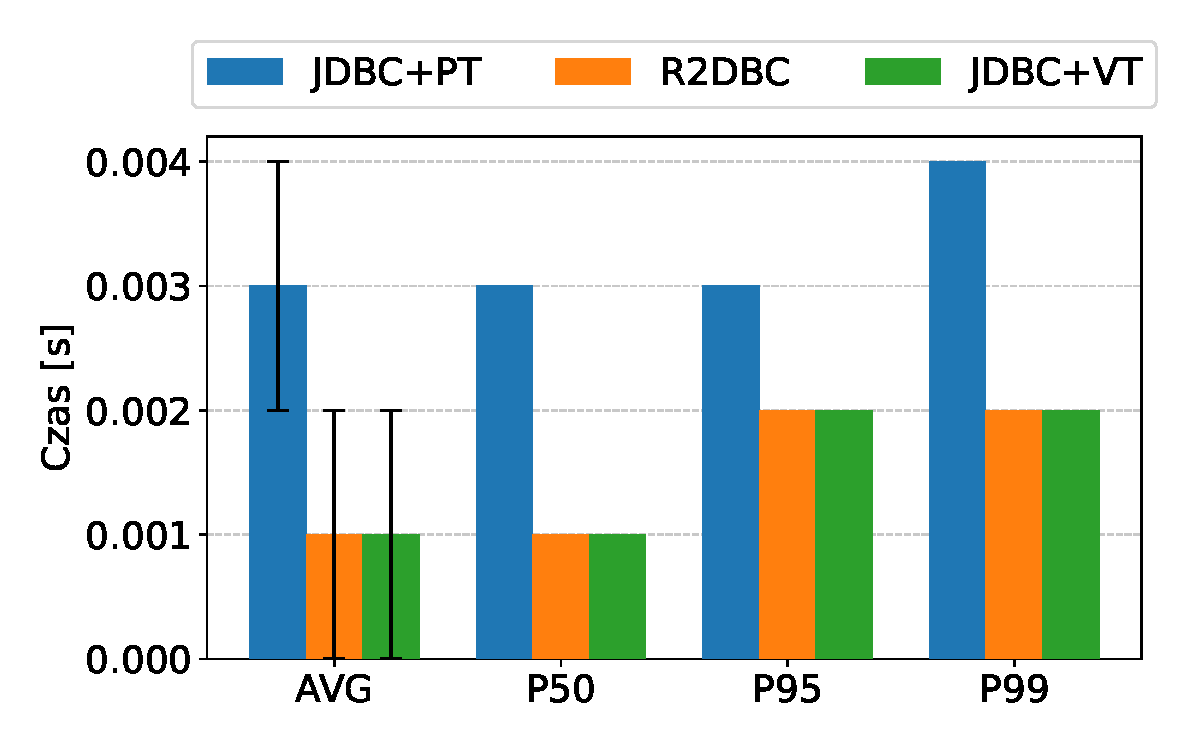
\includegraphics[width=\textwidth]{rozdzialy/rozdzial6/wykresy/A_plot_avg_Q1_16.pdf}
        \caption{poziom współbieżności: 16}
        \label{fig:benchmark-A-sample-Q1-16}
    \end{subfigure}
    \hfill
    \begin{subfigure}[b]{0.49\textwidth}
        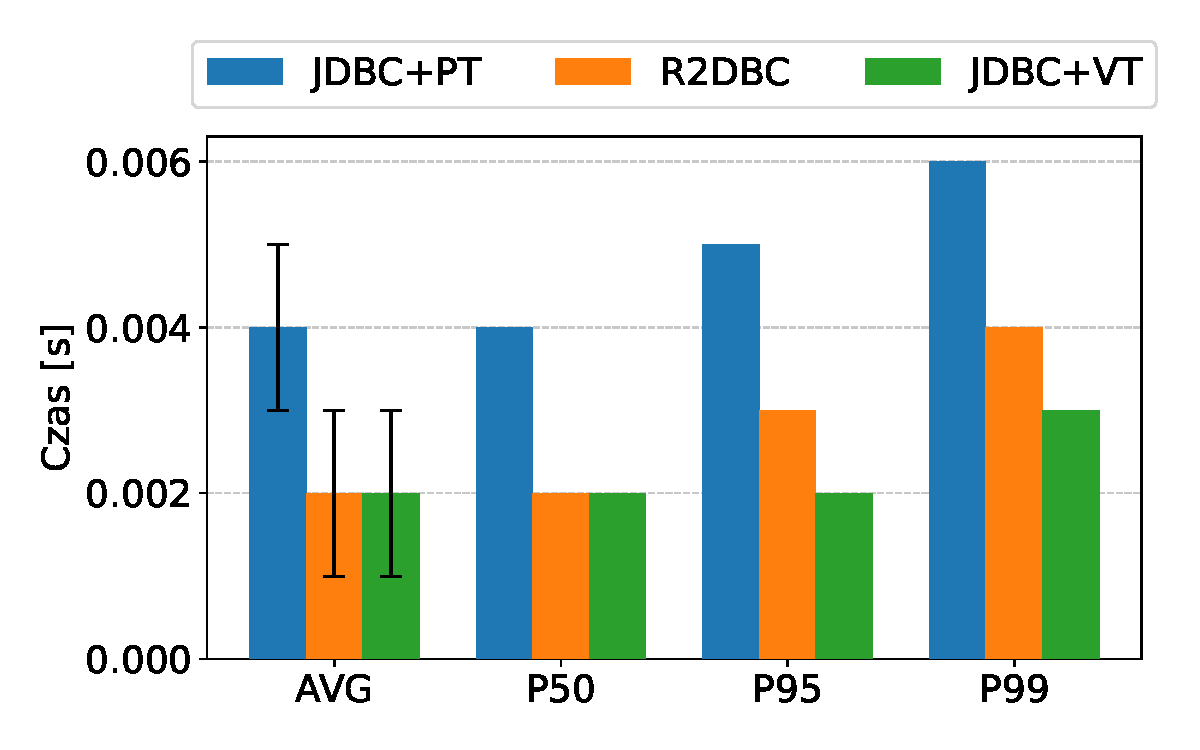
\includegraphics[width=\textwidth]{rozdzialy/rozdzial6/wykresy/A_plot_avg_Q1_32.pdf}
        \caption{poziom współbieżności: 32}
        \label{fig:benchmark-A-sample-Q1-32}
    \end{subfigure}

    \vspace{0.5cm}

    \begin{subfigure}[b]{0.49\textwidth}
        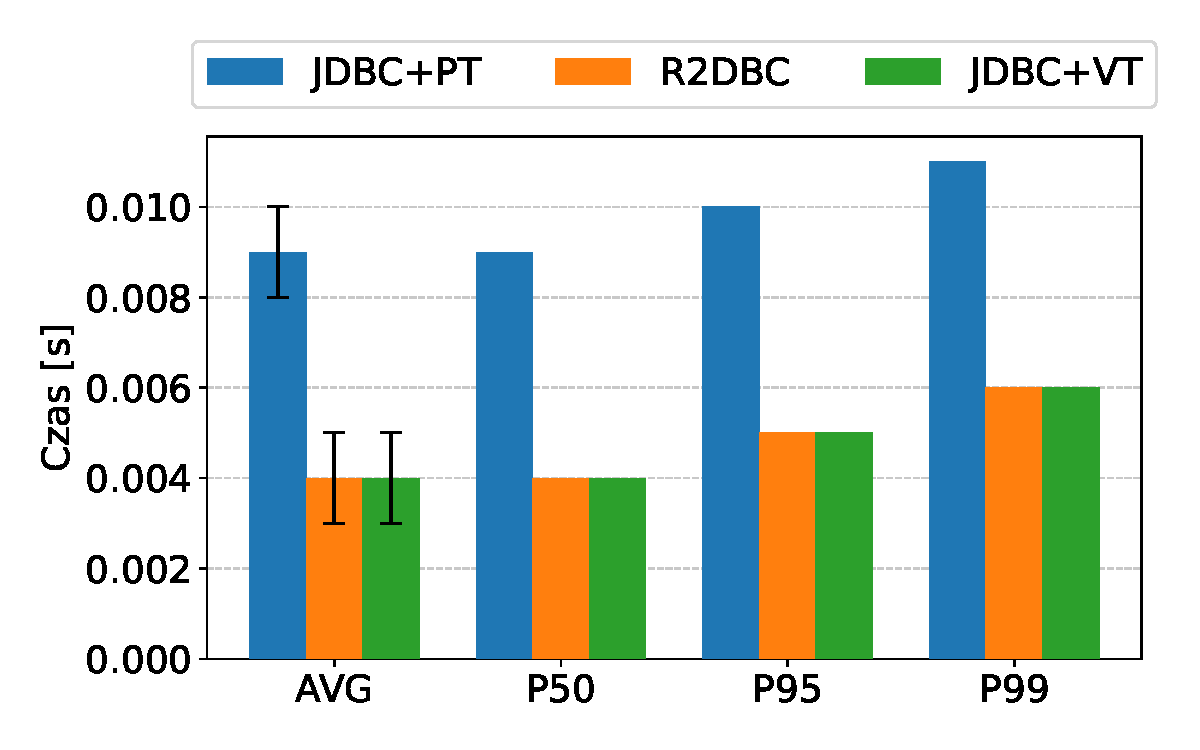
\includegraphics[width=\textwidth]{rozdzialy/rozdzial6/wykresy/A_plot_avg_Q1_64.pdf}
        \caption{poziom współbieżności: 64}
        \label{fig:benchmark-A-sample-Q1-64}
    \end{subfigure}
    \hfill
    \begin{subfigure}[b]{0.49\textwidth}
        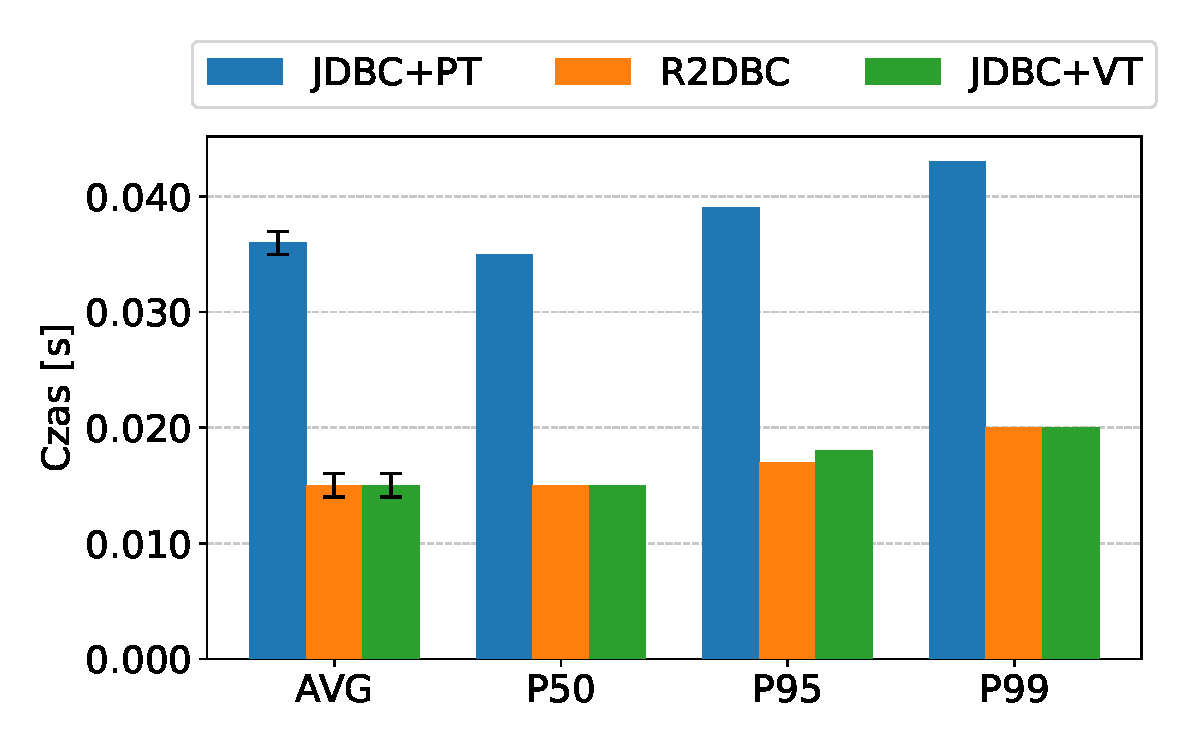
\includegraphics[width=\textwidth]{rozdzialy/rozdzial6/wykresy/A_plot_avg_Q1_256.pdf}
        \caption{poziom współbieżności: 256}
        \label{fig:benchmark-A-sample-Q1-256}
    \end{subfigure}

    \vspace{0.5cm}

    \begin{subfigure}[b]{0.49\textwidth}
        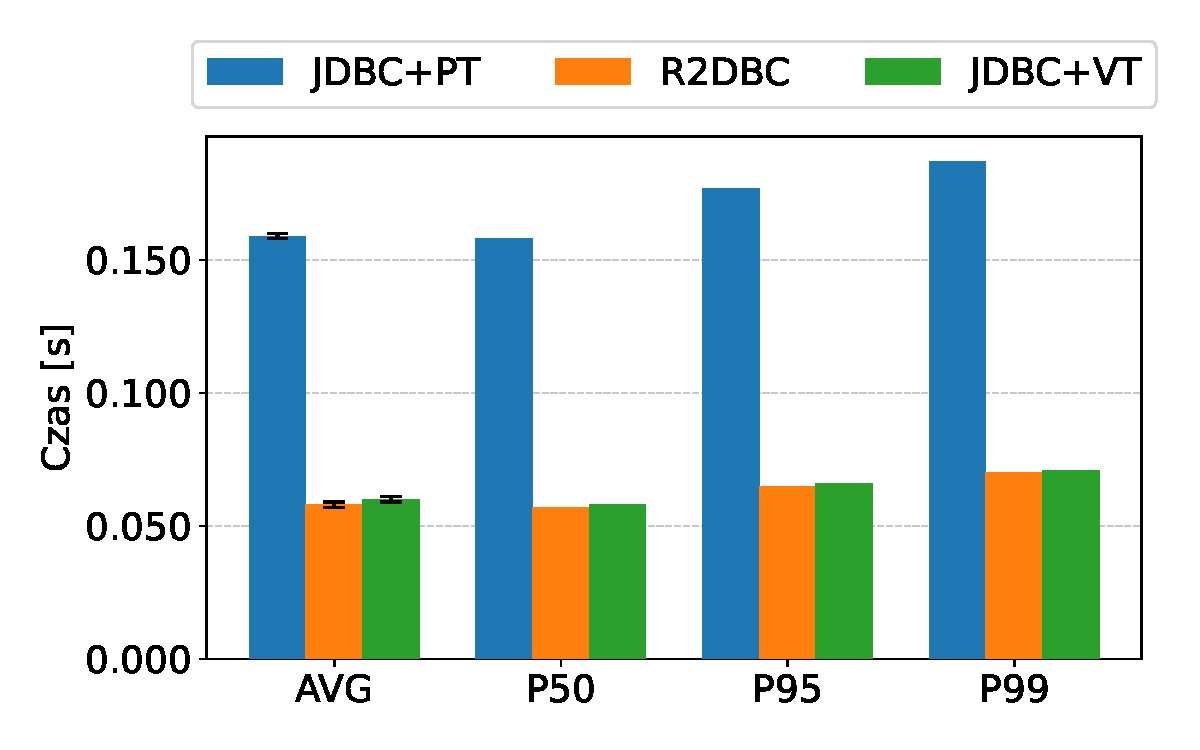
\includegraphics[width=\textwidth]{rozdzialy/rozdzial6/wykresy/A_plot_avg_Q1_1024.pdf}
        \caption{poziom współbieżności: 1024}
        \label{fig:benchmark-A-sample-Q1-1024}
    \end{subfigure}
    \caption{Wykresy kolumnowe średniego czasu i percentyli P50, P95, P99 dla zapytania \texttt{Q1} w~ramach scenariusza $\mathcal{A}$ w~zależności od poziomu współbieżności i~wariantu modelu współbieżności}
    \source{opracowanie własne}
    \label{fig:benchmark-A-sample-Q1}
\end{figure}

\setlength{\tabcolsep}{0.5em} % for the horizontal padding
\renewcommand{\arraystretch}{1.2} % for the vertical padding
\begin{table}[p]
    \centering
    \begin{tabularx}{\linewidth}{|c|c|>{\centering\arraybackslash}X|>{\centering\arraybackslash}X|>{\centering\arraybackslash}X|}
        \hline
        \textbf{Poz. współb.} & \textbf{Metryka} & \textbf{JDBC + PT} & \textbf{R2DBC} & \textbf{JDBC + VT} \\
        \hline
        \multirow{4}{*}{16} & AVG & $0.007 \pm 0.001$ & $0.006 \pm 0.001$ & $0.006 \pm 0.001$ \\ \cline{2-5}
                            & P50 & 0.008 & 0.007 & 0.007 \\ \cline{2-5}
                            & P95 & 0.010 & 0.008 & 0.008 \\ \cline{2-5}
                            & P99 & 0.012 & 0.010 & 0.011 \\
        \hline
        \multirow{4}{*}{32} & AVG & $0.010 \pm 0.001$ & $0.007 \pm 0.001$ & $0.007 \pm 0.001$ \\ \cline{2-5}
                            & P50 & 0.010 & 0.008 & 0.008 \\ \cline{2-5}
                            & P95 & 0.011 & 0.009 & 0.009 \\ \cline{2-5}
                            & P99 & 0.014 & 0.011 & 0.011 \\
        \hline
        \multirow{4}{*}{64} & AVG & $0.019 \pm 0.001$ & $0.013 \pm 0.001$ & $0.014 \pm 0.001$ \\ \cline{2-5}
                            & P50 & 0.019 & 0.014 & 0.014 \\ \cline{2-5}
                            & P95 & 0.021 & 0.016 & 0.016 \\ \cline{2-5}
                            & P99 & 0.025 & 0.020 & 0.022 \\
        \hline
        \multirow{4}{*}{256} & AVG & $0.068 \pm 0.001$ & $0.054 \pm 0.001$ & $0.053 \pm 0.001$ \\ \cline{2-5}
                             & P50 & 0.071 & 0.054 & 0.052 \\ \cline{2-5}
                             & P95 & 0.077 & 0.059 & 0.056 \\ \cline{2-5}
                             & P99 & 0.096 & 0.081 & 0.079 \\
        \hline
        \multirow{4}{*}{1024} & AVG & $0.297 \pm 0.003$ & $0.214 \pm 0.001$ & $0.200 \pm 0.002$ \\ \cline{2-5}
                              & P50 & 0.299 & 0.212 & 0.202 \\ \cline{2-5}
                              & P95 & 0.329 & 0.236 & 0.223 \\ \cline{2-5}
                              & P99 & 0.364 & 0.264 & 0.257 \\
        \hline
    \end{tabularx}
    \caption{Wartości średniego czasu i percentyli P50, P95, P99 dla zapytania \texttt{Q2} w~ramach scenariusza $\mathcal{A}$ w~zależności od poziomu współbieżności i~wariantu modelu współbieżności}
    \source{opracowanie własne}
    \label{table:benchmark-A-sample-Q2}
\end{table}

\begin{figure}[p]
    \centering
    \begin{subfigure}[b]{0.49\textwidth}
        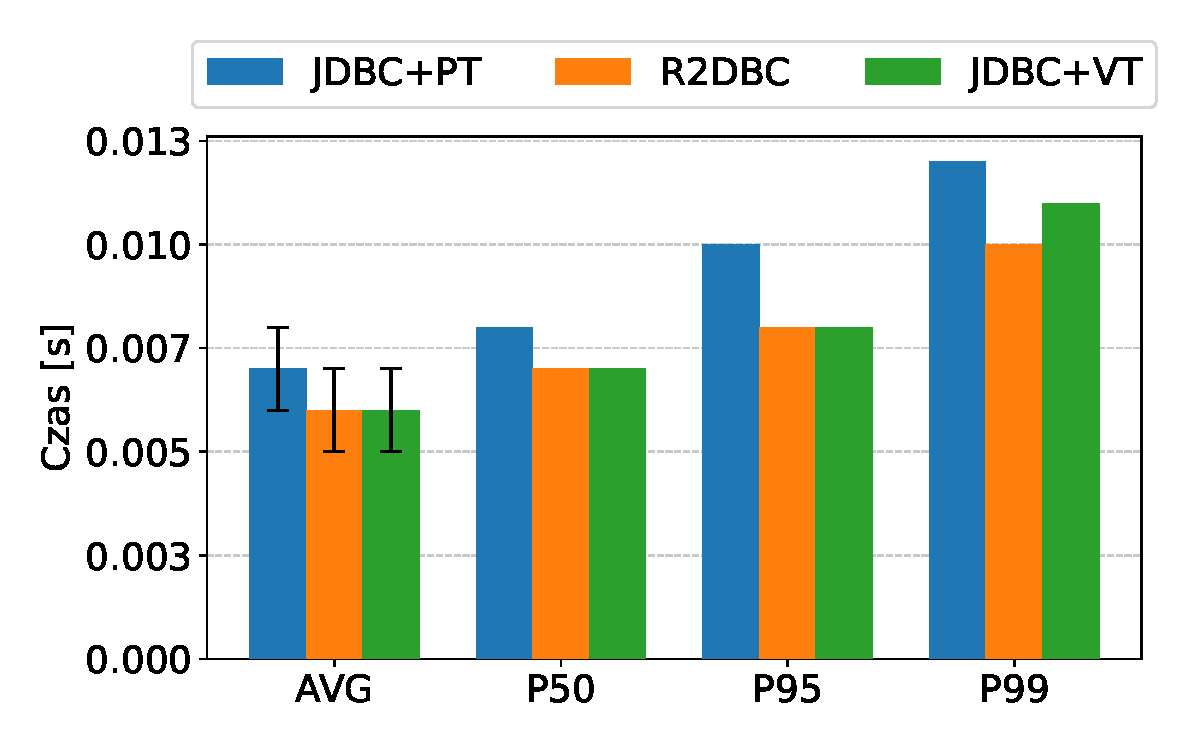
\includegraphics[width=\textwidth]{rozdzialy/rozdzial6/wykresy/A_plot_avg_Q2_16.pdf}
        \caption{poziom współbieżności: 16}
        \label{fig:benchmark-A-sample-Q2-16}
    \end{subfigure}
    \hfill
    \begin{subfigure}[b]{0.49\textwidth}
        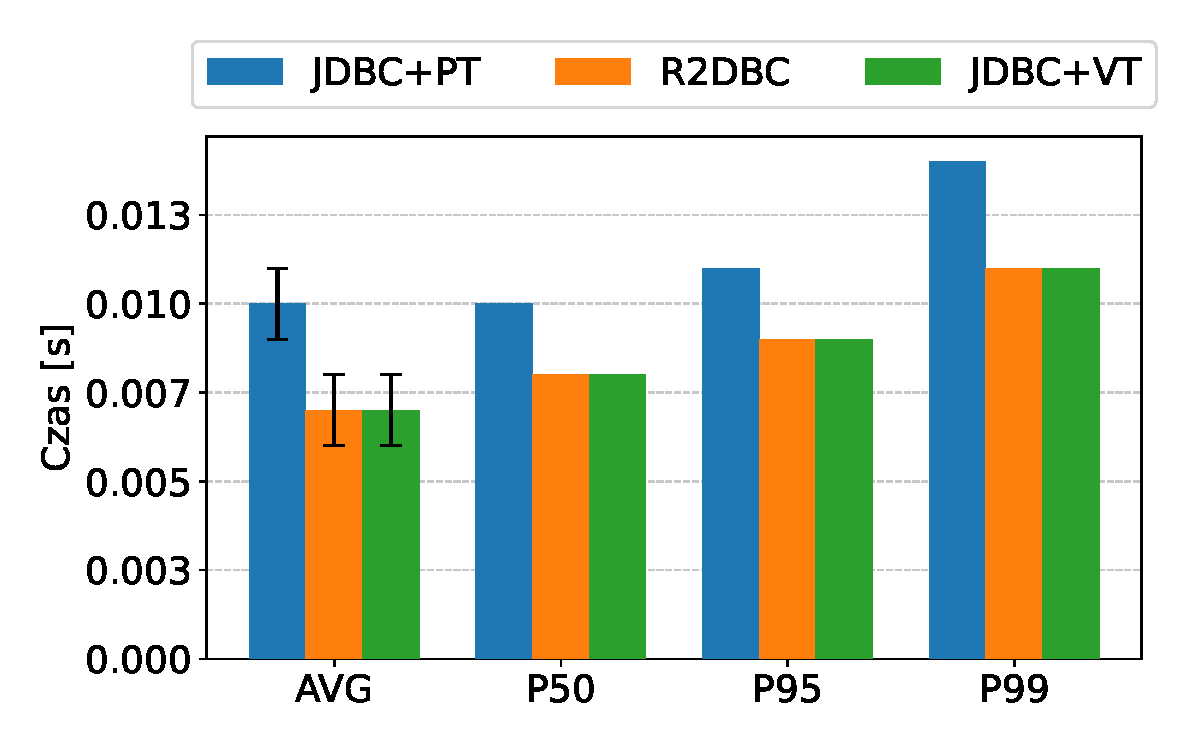
\includegraphics[width=\textwidth]{rozdzialy/rozdzial6/wykresy/A_plot_avg_Q2_32.pdf}
        \caption{poziom współbieżności: 32}
        \label{fig:benchmark-A-sample-Q2-32}
    \end{subfigure}

    \vspace{0.5cm}

    \begin{subfigure}[b]{0.49\textwidth}
        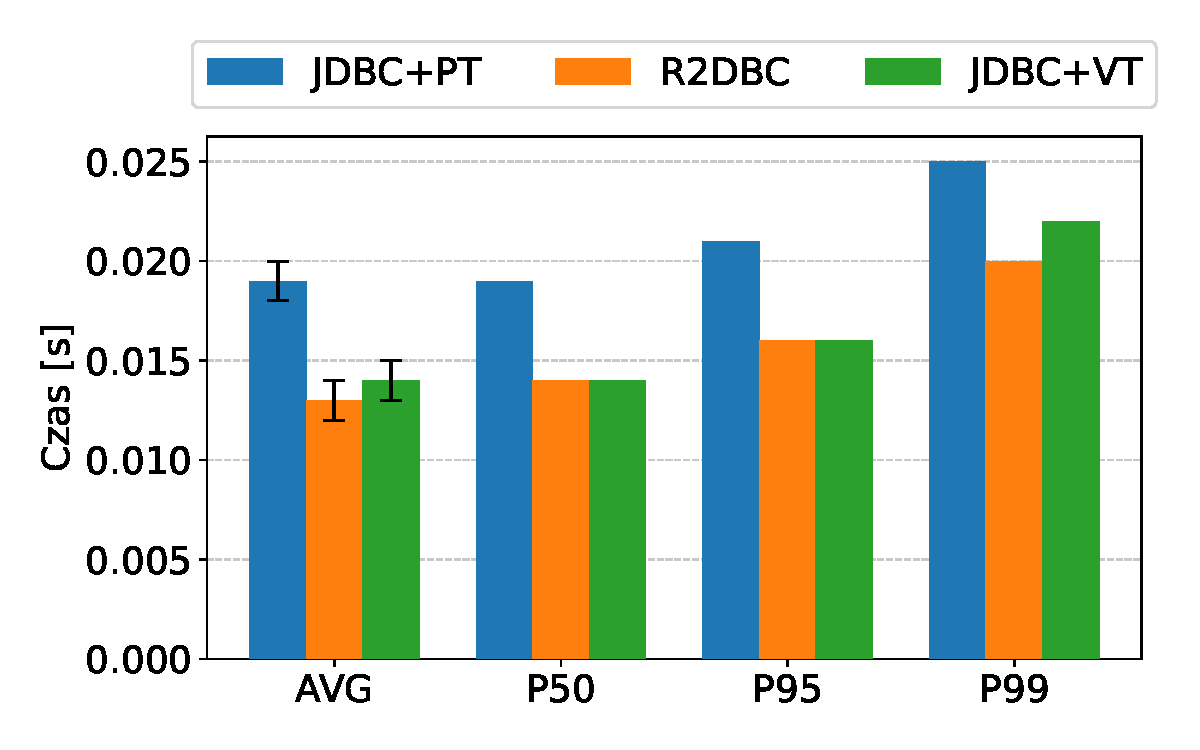
\includegraphics[width=\textwidth]{rozdzialy/rozdzial6/wykresy/A_plot_avg_Q2_64.pdf}
        \caption{poziom współbieżności: 64}
        \label{fig:benchmark-A-sample-Q2-64}
    \end{subfigure}
    \hfill
    \begin{subfigure}[b]{0.49\textwidth}
        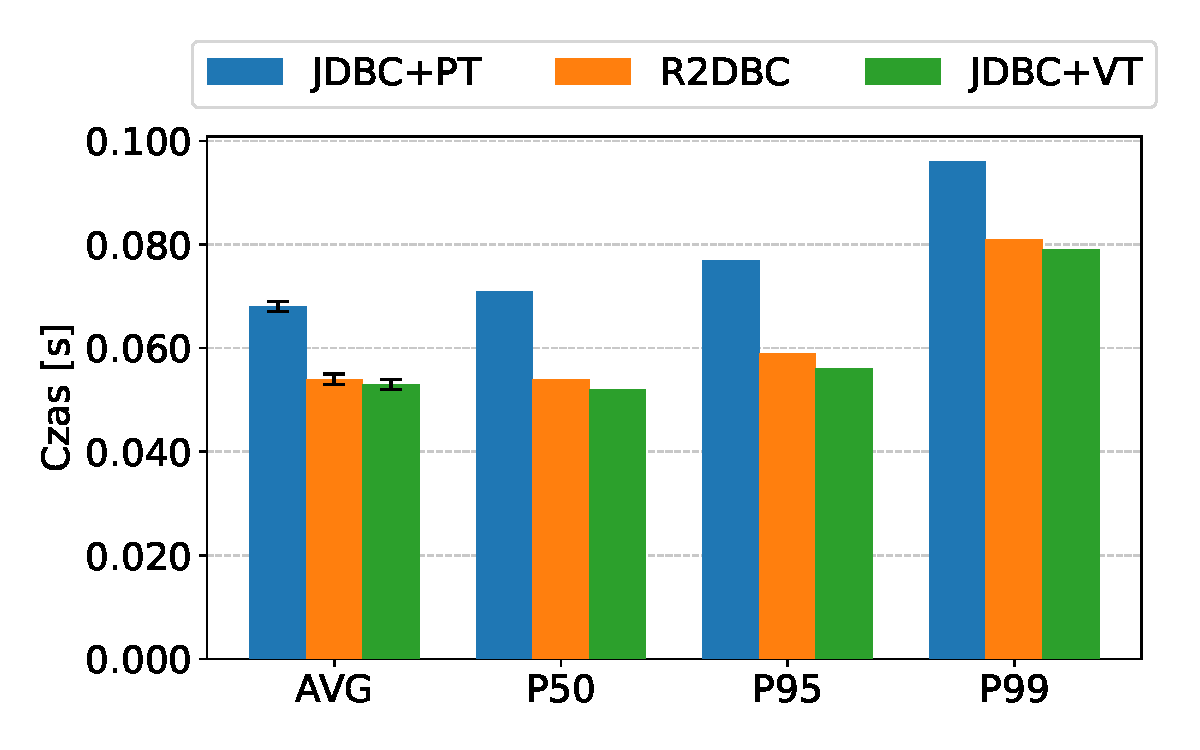
\includegraphics[width=\textwidth]{rozdzialy/rozdzial6/wykresy/A_plot_avg_Q2_256.pdf}
        \caption{poziom współbieżności: 256}
        \label{fig:benchmark-A-sample-Q2-256}
    \end{subfigure}

    \vspace{0.5cm}

    \begin{subfigure}[b]{0.49\textwidth}
        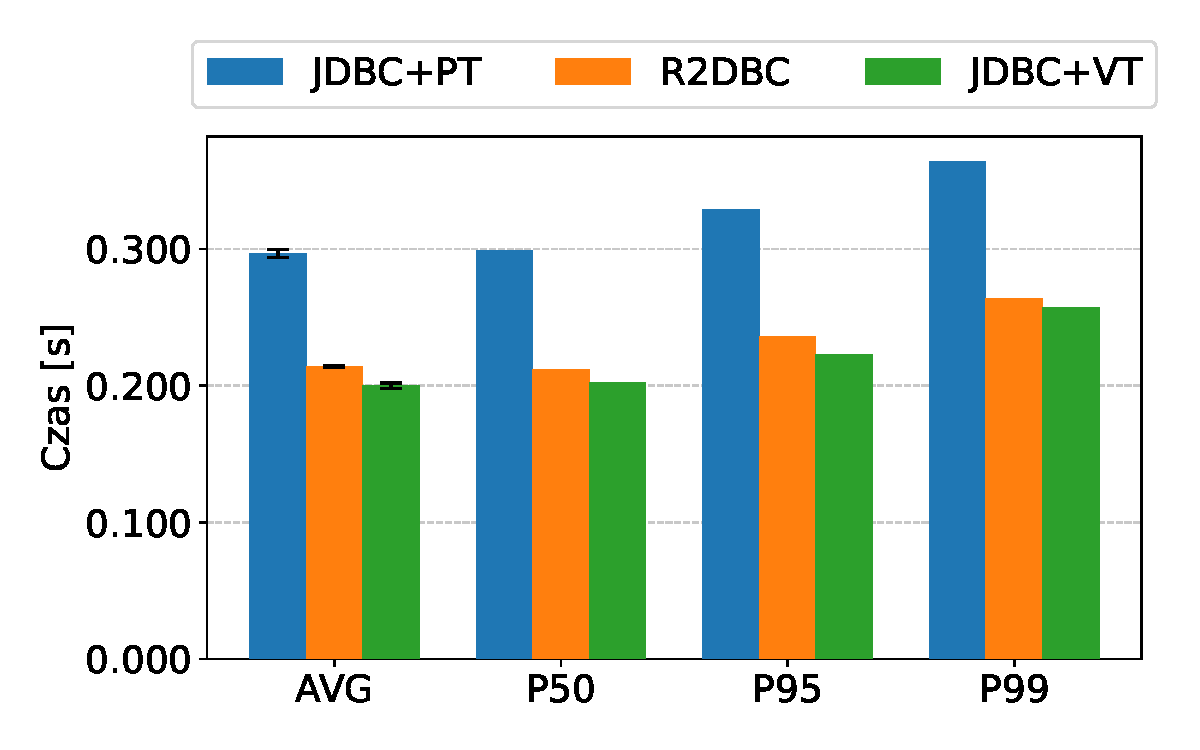
\includegraphics[width=\textwidth]{rozdzialy/rozdzial6/wykresy/A_plot_avg_Q2_1024.pdf}
        \caption{poziom współbieżności: 1024}
        \label{fig:benchmark-A-sample-Q2-1024}
    \end{subfigure}
    \caption{Wykresy kolumnowe średniego czasu i percentyli P50, P95, P99 dla zapytania \texttt{Q2} w~ramach scenariusza $\mathcal{A}$ w~zależności od poziomu współbieżności i~wariantu modelu współbieżności}
    \source{opracowanie własne}
    \label{fig:benchmark-A-sample-Q2}
\end{figure}

\setlength{\tabcolsep}{0.5em} % for the horizontal padding
\renewcommand{\arraystretch}{1.2} % for the vertical padding
\begin{table}[p]
    \centering
    \begin{tabularx}{\linewidth}{|c|c|>{\centering\arraybackslash}X|>{\centering\arraybackslash}X|>{\centering\arraybackslash}X|}
        \hline
        \textbf{Poz. współb.} & \textbf{Metryka} & \textbf{JDBC + PT} & \textbf{R2DBC} & \textbf{JDBC + VT} \\
        \hline
        \multirow{4}{*}{16} & AVG & $0.202 \pm 0.001$ & $0.200 \pm 0.001$ & $0.202 \pm 0.001$ \\ \cline{2-5}
                            & P50 & 0.200 & 0.199 & 0.200 \\ \cline{2-5}
                            & P95 & 0.217 & 0.216 & 0.218 \\ \cline{2-5}
                            & P99 & 0.227 & 0.226 & 0.228 \\
        \hline
        \multirow{4}{*}{32} & AVG & $0.374 \pm 0.001$ & $0.372 \pm 0.001$ & $0.374 \pm 0.001$ \\ \cline{2-5}
                            & P50 & 0.371 & 0.369 & 0.372 \\ \cline{2-5}
                            & P95 & 0.400 & 0.394 & 0.394 \\ \cline{2-5}
                            & P99 & 0.412 & 0.412 & 0.406 \\
        \hline
        \multirow{4}{*}{64} & AVG & $0.757 \pm 0.003$ & $0.751 \pm 0.003$ & $0.760 \pm 0.003$ \\ \cline{2-5}
                            & P50 & 0.753 & 0.748 & 0.755 \\ \cline{2-5}
                            & P95 & 0.784 & 0.778 & 0.793 \\ \cline{2-5}
                            & P99 & 0.820 & 0.820 & 0.830 \\
        \hline
        \multirow{4}{*}{256} & AVG & $3.023 \pm 0.012$ & $2.999 \pm 0.016$ & $3.007 \pm 0.013$ \\ \cline{2-5}
                             & P50 & 3.012 & 2.991 & 3.001 \\ \cline{2-5}
                             & P95 & 3.091 & 3.078 & 3.095 \\ \cline{2-5}
                             & P99 & 3.176 & 3.311 & 3.148 \\
        \hline
        \multirow{4}{*}{1024} & AVG & $5.336 \pm 0.010$ & $11.954 \pm 0.054$ & $5.206 \pm 0.009$ \\ \cline{2-5}
                              & P50 & 5.335 & 11.929 & 5.201 \\ \cline{2-5}
                              & P95 & 5.377 & 12.148 & 5.234 \\ \cline{2-5}
                              & P99 & 5.385 & 12.231 & 5.260 \\
        \hline
    \end{tabularx}
    \caption{Wartości średniego czasu i percentyli P50, P95, P99 dla zapytania \texttt{Q3} w~ramach scenariusza $\mathcal{A}$ w~zależności od poziomu współbieżności i~wariantu modelu współbieżności}
    \source{opracowanie własne}
    \label{table:benchmark-A-sample-Q3}
\end{table}

% \begin{figure}[ht]
%     \centering
%     \includegraphics[width=\textwidth]{rozdzialy/rozdzial6/wykresy/A_plot_avg_Q3.pdf}
%     \caption{Wykres kolumnowy średniego czasu zapytania \texttt{Q3} w zależności od poziomu współbieżności i wariantu modelu współbieżności}
%     \source{opracowanie własne}
%     \label{fig:benchmark-avg-q3}
% \end{figure}

\begin{figure}[p]
    \centering
    \begin{subfigure}[b]{0.49\textwidth}
        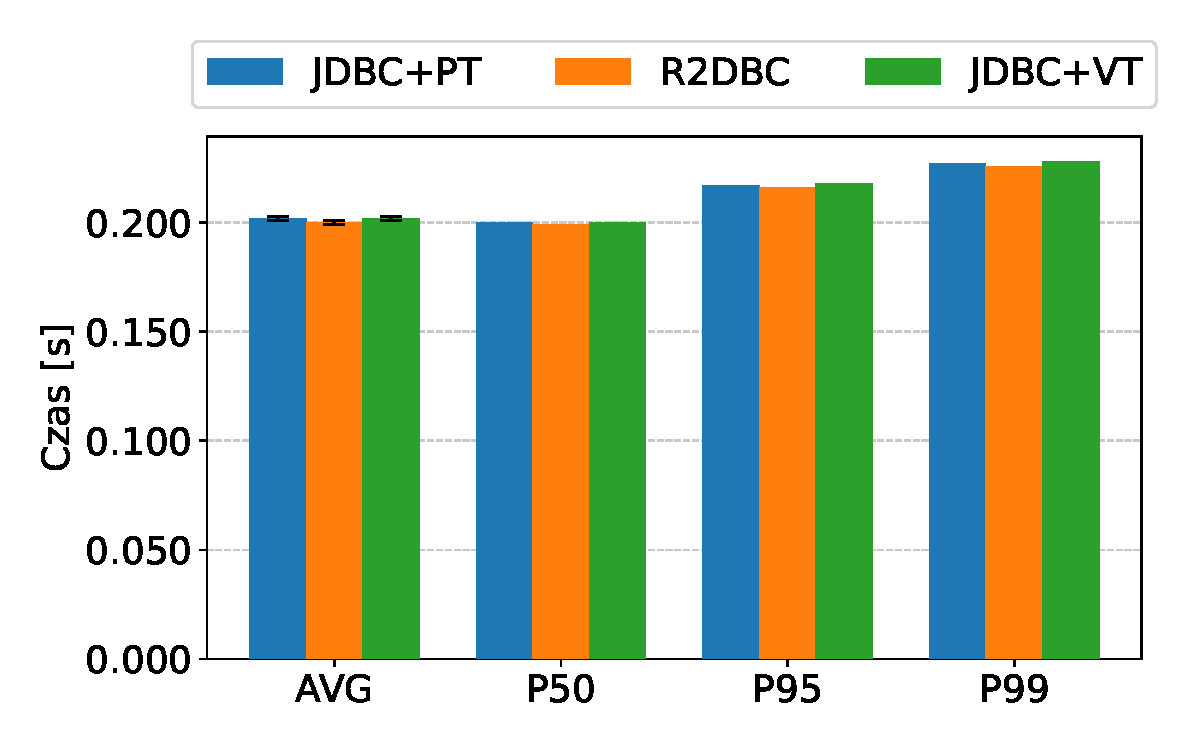
\includegraphics[width=\textwidth]{rozdzialy/rozdzial6/wykresy/A_plot_avg_Q3_16.pdf}
        \caption{poziom współbieżności: 16}
        \label{fig:benchmark-A-sample-Q3-16}
    \end{subfigure}
    \hfill
    \begin{subfigure}[b]{0.49\textwidth}
        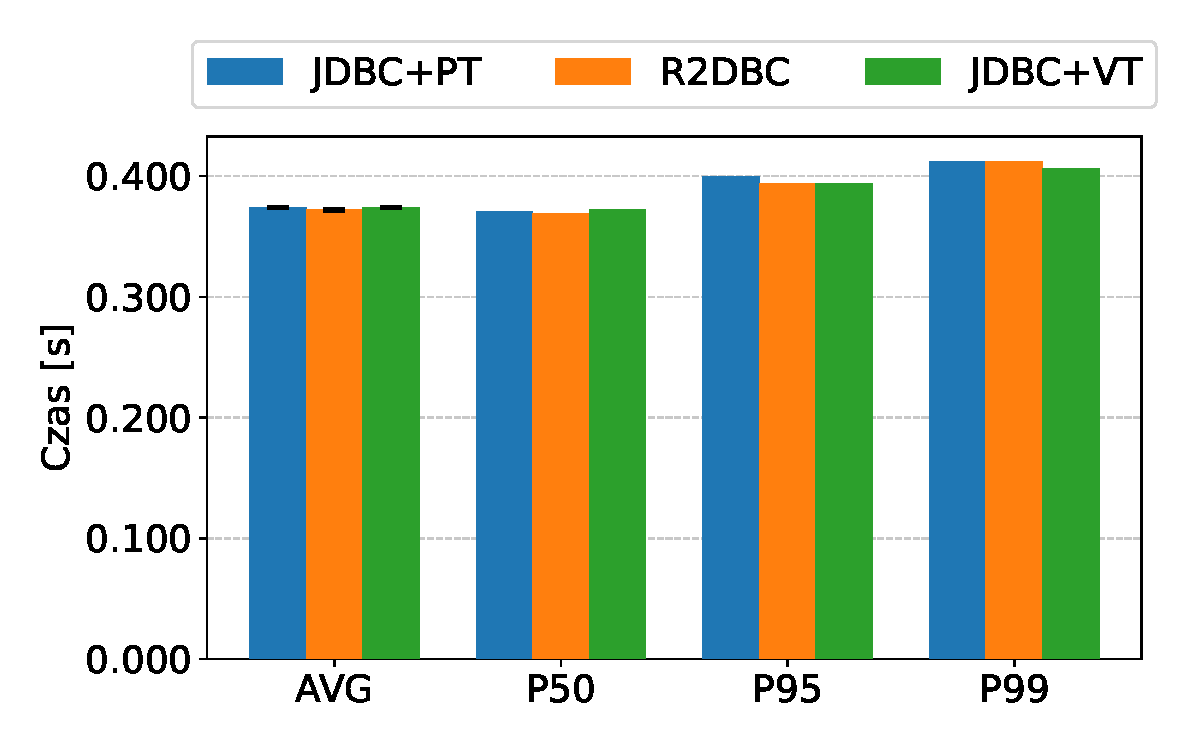
\includegraphics[width=\textwidth]{rozdzialy/rozdzial6/wykresy/A_plot_avg_Q3_32.pdf}
        \caption{poziom współbieżności: 32}
        \label{fig:benchmark-A-sample-Q3-32}
    \end{subfigure}

    \vspace{0.5cm}

    \begin{subfigure}[b]{0.49\textwidth}
        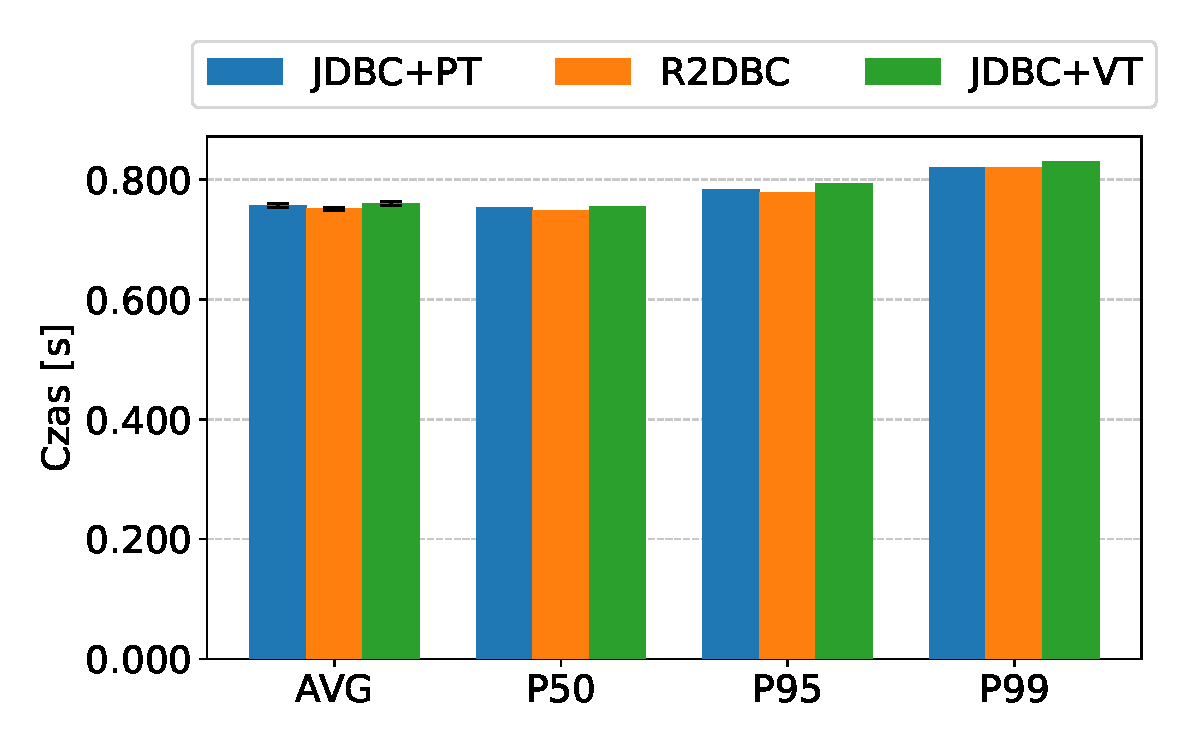
\includegraphics[width=\textwidth]{rozdzialy/rozdzial6/wykresy/A_plot_avg_Q3_64.pdf}
        \caption{poziom współbieżności: 64}
        \label{fig:benchmark-A-sample-Q3-64}
    \end{subfigure}
    \hfill
    \begin{subfigure}[b]{0.49\textwidth}
        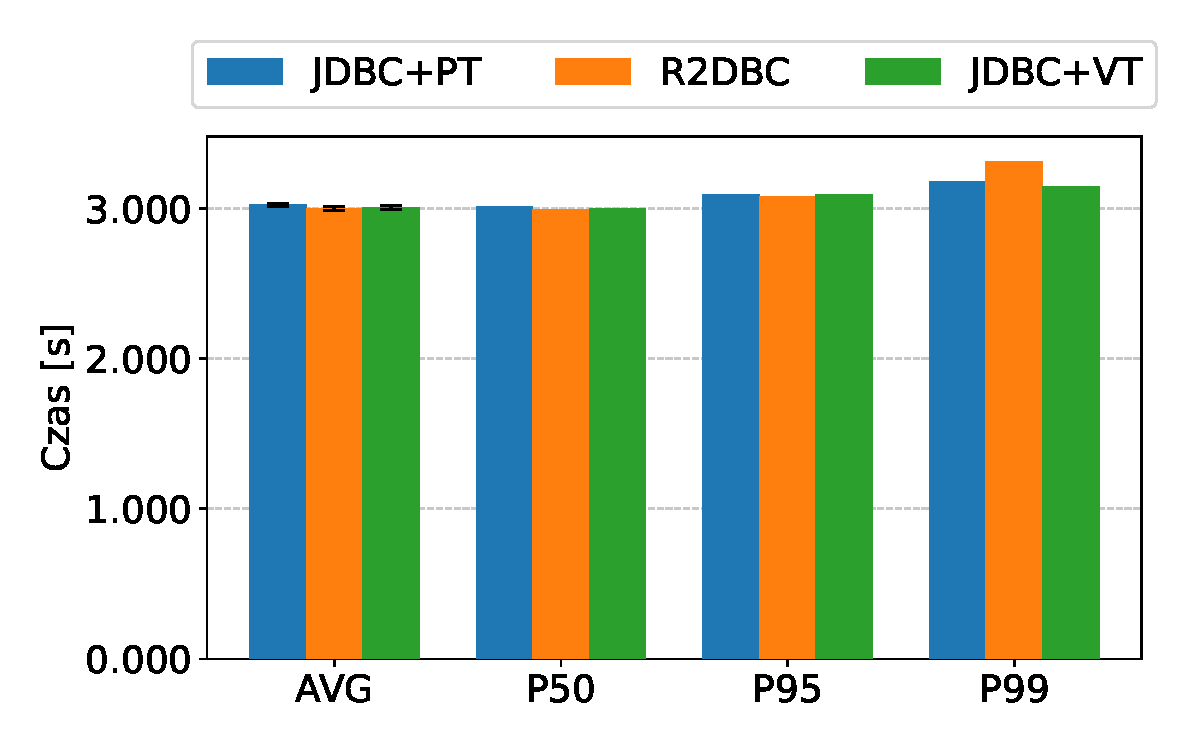
\includegraphics[width=\textwidth]{rozdzialy/rozdzial6/wykresy/A_plot_avg_Q3_256.pdf}
        \caption{poziom współbieżności: 256}
        \label{fig:benchmark-A-sample-Q3-256}
    \end{subfigure}

    \vspace{0.5cm}

    \begin{subfigure}[b]{0.49\textwidth}
        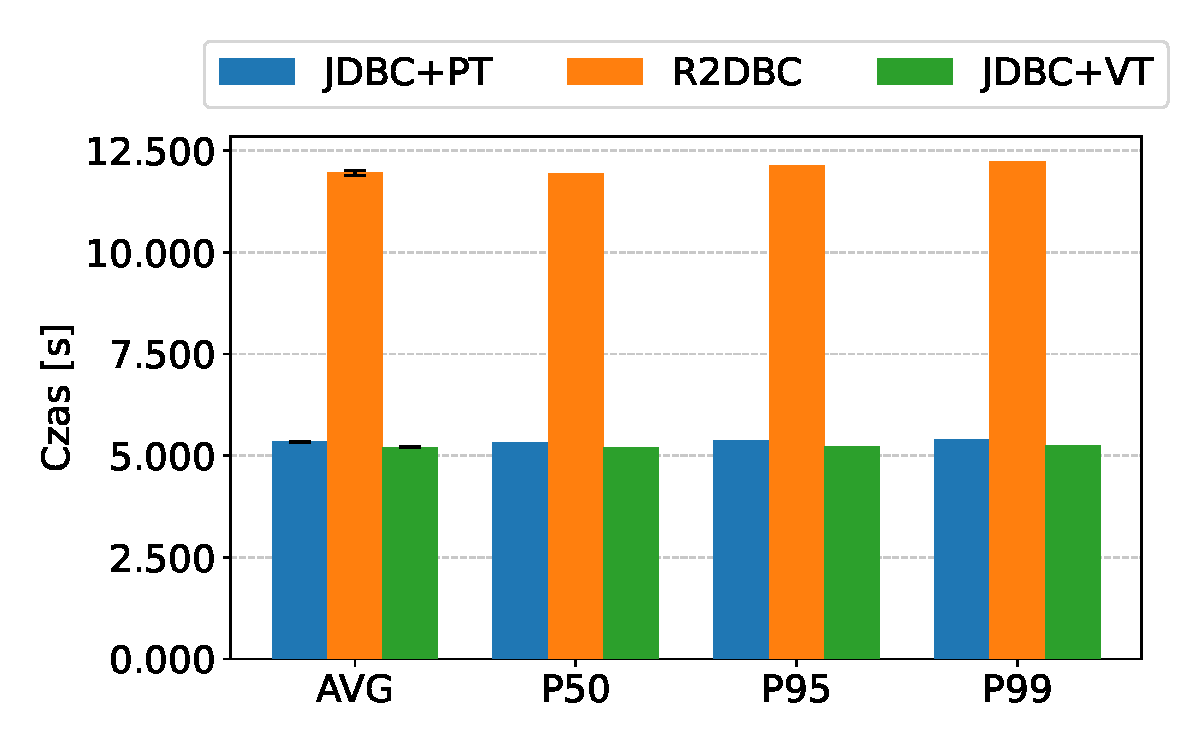
\includegraphics[width=\textwidth]{rozdzialy/rozdzial6/wykresy/A_plot_avg_Q3_1024.pdf}
        \caption{poziom współbieżności: 1024}
        \label{fig:benchmark-A-sample-Q3-1024}
    \end{subfigure}
    \caption{Wykresy kolumnowe średniego czasu i percentyli P50, P95, P99 dla zapytania \texttt{Q3} w~ramach scenariusza $\mathcal{A}$ w~zależności od poziomu współbieżności i~wariantu modelu współbieżności}
    \source{opracowanie własne}
    \label{fig:benchmark-A-sample-Q3}
\end{figure}

\newpage
\subsection{Wyniki pomiarów w ramach scenariusza \ensuremath{\mathcal{B}}}
\label{sec:results-scenario-B}

\subsubsection{Tryb próbkowania czasu (\texttt{SampleTime})}
bla bla bla

\vspace{3cm}
\textit{Wyniki znajdują się na następnej stronie.}

\setlength{\tabcolsep}{0.5em} % for the horizontal padding
\renewcommand{\arraystretch}{1.2} % for the vertical padding
\begin{table}[p]
    \centering
    \begin{tabularx}{\linewidth}{|c|c|>{\centering\arraybackslash}X|>{\centering\arraybackslash}X|>{\centering\arraybackslash}X|}
        \hline
        \textbf{Wariant serwisów} & \textbf{Metryka} & \textbf{Legacy} & \textbf{Reactive} & \textbf{Loom} \\
        \hline
        \multirow{5}{*}{\texttt{THREE\_FAST\_TWO\_SLOW}} & AVG & $0.040 \pm 0.001$ & $0.013 \pm 0.001$ & $0.014 \pm 0.001$ \\ \cline{2-5}
                            & P50   & 0.036 & 0.011 & 0.011 \\ \cline{2-5}
                            & P95   & 0.075 & 0.041 & 0.041 \\ \cline{2-5}
                            & P99   & 0.092 & 0.041 & 0.042 \\ \cline{2-5}
                            & P99.9 & 0.119 & 0.042 & 0.042 \\
        \hline
        \multirow{5}{*}{\texttt{ONE\_FAST\_FOUR\_SLOW}} & AVG & $0.117 \pm 0.003$ & $0.091 \pm 0.001$ & $0.092 \pm 0.001$ \\ \cline{2-5}
                            & P50   & 0.107 & 0.091 & 0.091 \\ \cline{2-5}
                            & P95   & 0.250 & 0.111 & 0.111 \\ \cline{2-5}
                            & P99   & 0.251 & 0.120 & 0.120 \\ \cline{2-5}
                            & P99.9 & 0.252 & 0.216 & 0.217 \\
        \hline
        \multirow{5}{*}{\texttt{FIVE\_SIMILAR}} & AVG & $0.053 \pm 0.001$ & $0.039 \pm 0.001$ & $0.039 \pm 0.001$ \\ \cline{2-5}
                            & P50   & 0.045 & 0.038 & 0.039 \\ \cline{2-5}
                            & P95   & 0.150 & 0.045 & 0.045 \\ \cline{2-5}
                            & P99   & 0.151 & 0.048 & 0.048 \\ \cline{2-5}
                            & P99.9 & 0.153 & 0.051 & 0.052 \\
        \hline
        \multirow{5}{*}{\texttt{OUTLIER\_HEAVY}} & AVG & $0.166 \pm 0.010$ & $0.050 \pm 0.003$ & $0.051 \pm 0.003$ \\ \cline{2-5}
                             & P50   & 0.058 & 0.037 & 0.037 \\ \cline{2-5}
                             & P95   & 0.301 & 0.300 & 0.300 \\ \cline{2-5}
                             & P99   & 0.324 & 0.301 & 0.301 \\ \cline{2-5}
                             & P99.9 & 0.341 & 0.302 & 0.302 \\
        \hline
    \end{tabularx}
    \caption{Wartości średniego czasu i percentyli P50, P95, P99, P99.9 dla scenariusza $\mathcal{B}$ w~zależności od wariantu serwisów i~modelu współbieżności}
    \source{opracowanie własne}
    \label{table:benchmark-B-sample}
\end{table}

% \begin{figure}[ht]
%     \centering
%     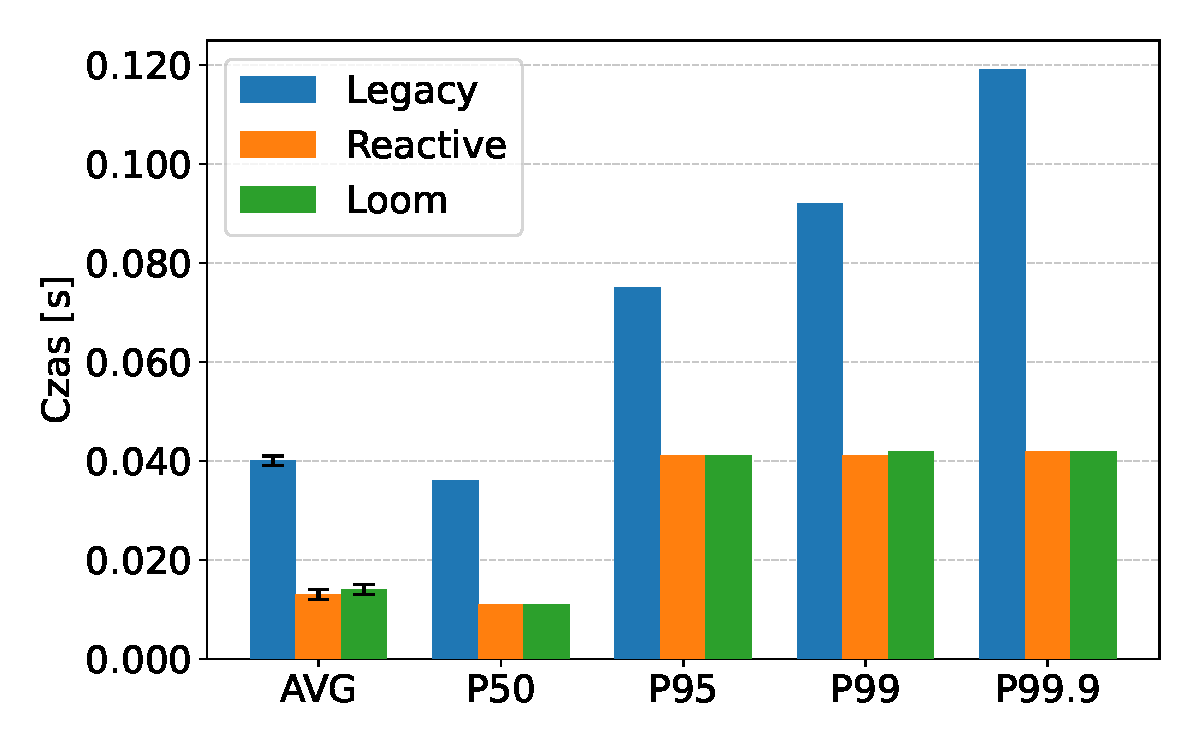
\includegraphics[width=\textwidth]{rozdzialy/rozdzial6/wykresy/B_plot_avg_C1.pdf}
%     \caption{Wykres kolumnowy średniego czasu i latencji P50, P95, P99 i P99.9 dla różnych modeli współbieżności w scenariuszu B dla wariantu \texttt{THREE\_FAST\_TWO\_SLOW}}
%     \source{opracowanie własne}
%     \label{fig:benchmark-B-sample-C1}
% \end{figure}

\begin{figure}[p]
    \centering
    \begin{subfigure}[b]{0.49\textwidth}
        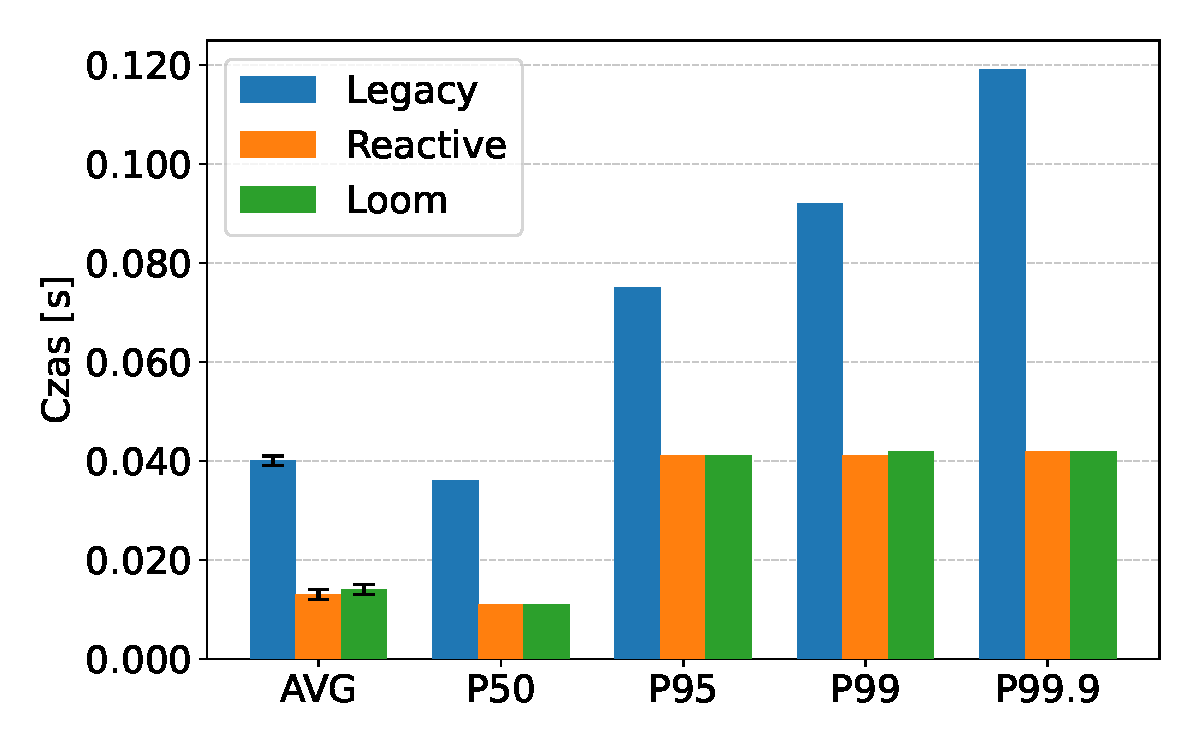
\includegraphics[width=\textwidth]{rozdzialy/rozdzial6/wykresy/B_plot_avg_C1.pdf}
        \caption{wariant \texttt{THREE\_FAST\_TWO\_SLOW}}
        \label{fig:benchmark-B-sample-C1}
    \end{subfigure}
    \hfill
    \begin{subfigure}[b]{0.49\textwidth}
        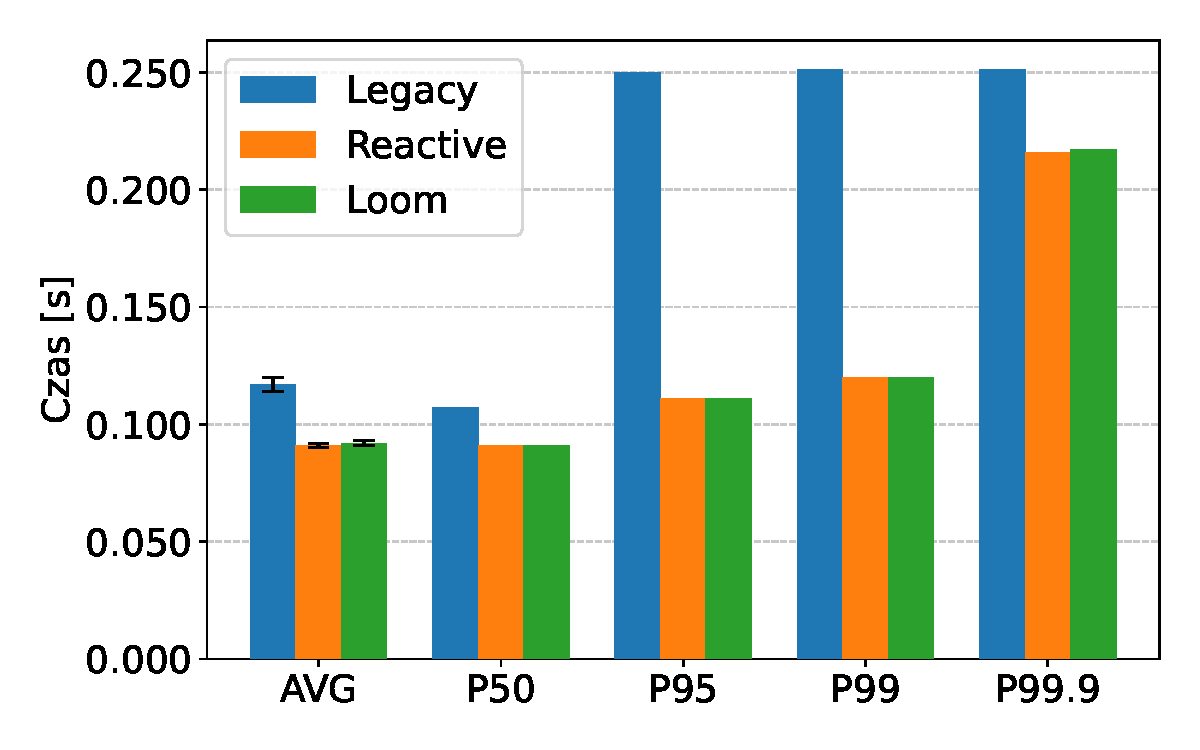
\includegraphics[width=\textwidth]{rozdzialy/rozdzial6/wykresy/B_plot_avg_C2.pdf}
        \caption{wariant \texttt{ONE\_FAST\_FOUR\_SLOW}}
        \label{fig:benchmark-B-sample-C2}
    \end{subfigure}

    \vspace{0.5cm}

    \begin{subfigure}[b]{0.49\textwidth}
        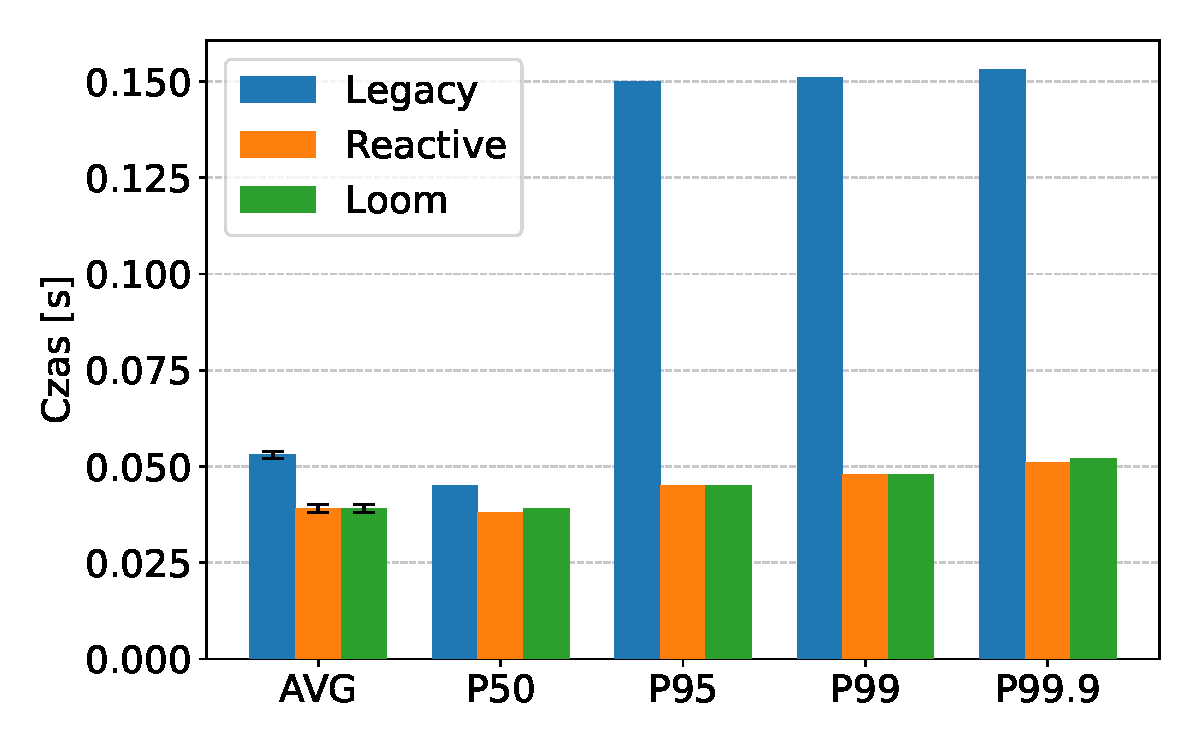
\includegraphics[width=\textwidth]{rozdzialy/rozdzial6/wykresy/B_plot_avg_C3.pdf}
        \caption{wariant \texttt{FIVE\_SIMILAR}}
        \label{fig:benchmark-B-sample-C3}
    \end{subfigure}
    \hfill
    \begin{subfigure}[b]{0.49\textwidth}
        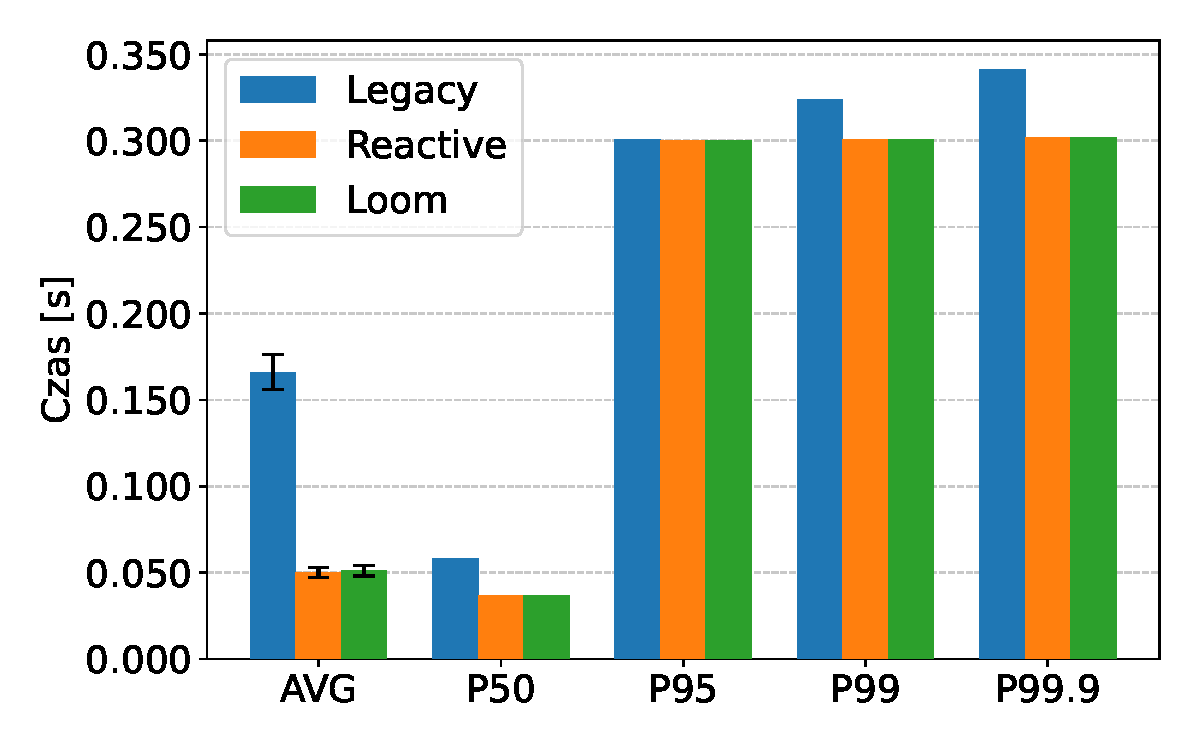
\includegraphics[width=\textwidth]{rozdzialy/rozdzial6/wykresy/B_plot_avg_C4.pdf}
        \caption{wariant \texttt{OUTLIER\_HEAVY}}
        \label{fig:benchmark-B-sample-C4}
    \end{subfigure}
    \caption{Wykresy kolumnowe średniego czasu i percentyli P50, P95, P99, P99.9 dla scenariusza $\mathcal{B}$ w~zależności od wariantu serwisów i~modelu współbieżności}
    \source{opracowanie własne}
    \label{fig:benchmark-B-sample}
\end{figure}

\newpage
\section{Analiza porównawcza i interpretacja wyników}

\subsection{Scenariusz \ensuremath{\mathcal{A}}}

\subsection{Scenariusz \ensuremath{\mathcal{B}}}
\cleardoublepage

\chapter{Wnioski i rekomendacje}

\section{Odpowiedzi na pytania badawcze}

\section{Rekomendacje i wzorce zastosowań mechanizmów Project Loom}

\section{Ograniczenia badań i propozycje dalszych badań}
\cleardoublepage

\chapter{Podsumowanie}

Stworzenie aplikacji \emph{Grocery Scanner} wymagało ogromnego nakładu czasowego. Proces jej powstawania był pełen różnych koncepcji i pomysłów na rozbudowę aplikacji. Wiele z~nich często podlegało zmianom, lecz efekt końcowy pozwala stwierdzić, że aplikacja spełnia wyrażone we wstępie założenia. Możliwe jest jednak poszerzanie jej o dodatkowe funkcjonalności. Przykładowymi planami na rozwój aplikacji są:

\begin{itemize}
    \item \emph{możliwość logowania i rejestracji za pomocą konta w takich serwisach, jak Google i~Facebook}, co~usprawni zaimplementowany już proces, a w konsekwencji pozwoli na powiększenie liczby użytkowników korzystających z aplikacji,
    \item \emph{system zgłaszania profili użytkowników}, który pozwoli na ograniczenie szkodliwej działalności w aplikacji poprzez ograniczanie lub blokowanie dostępu,
    \item \emph{rozszerzenie listy preferencji żywieniowych}, która ułatwi korzystanie z aplikacji większej liczbie użytkowników,
    \item \emph{pobieranie informacji o produktach z innych źródeł}, co pozwoli na wzrost jakości danych, a także w dużym stopniu ograniczy przypadki, w których aplikacja zwraca informację o braku danych skanowanego produktu.
\end{itemize}

\noindent
Warto zaznaczyć, że funkcjonalności zawarte w powyższej liście nie zostały zaimplementowane z uwagi na fakt, że wykraczały poza podstawowe założenia co do funkcjonalności aplikacji opisanych we wstępie pracy.
%  w małym stopniu przybliżały do zrealizowania podstawowych założeń aplikacji zawartych we wstępie, co było głównym celem.

Proces tworzenia niniejszej pracy przede wszystkim pozwolił na pogłębienie wiedzy. W~tej kwestii szczególną uwagę należy zwrócić uwagę na aspekt „techniczny”. Tworzenie aplikacji \emph{Grocery Scanner} pozwoliło na poznanie nieużywanych wcześniej przez autora pracy bibliotek i~narzędzi, jak również umożliwiło poszerzenie wiedzy na temat poznanych wcześniej rozwiązań. Sam proces tworzenia aplikacji na urządzenia mobilne okazał się być niezwykle pouczający, zarówno w kontekście poszerzania wiedzy technicznej, jak i rozwoju kariery zawodowej.
\cleardoublepage

\phantomsection\addcontentsline{toc}{chapter}{Bibliografia}
% \bibliographystyle{unsrt}
% \bibliography{bibliografia}
\printbibliography
\clearpage

\phantomsection\addcontentsline{toc}{chapter}{Spis rysunków}
\listoffigures
\clearpage

\phantomsection\addcontentsline{toc}{chapter}{Spis tabel}
\listoftables
\clearpage

\phantomsection\addcontentsline{toc}{chapter}{Spis kodów źródłowych}
\renewcommand\listoflistingscaption{Spis kodów źródłowych}
\listoflistings

\end{document}